\documentclass[12pt,aspectratio=169]{beamer}

% Input
\usepackage[utf8]{inputenc}
\usepackage[T1]{fontenc}
\usepackage[letterspace=100]{microtype}
\usepackage{upquote}

% Beamer
\usetheme{metropolis}
\usepackage[sfdefault]{FiraSans}
\usepackage{xcolor}
\definecolor{blue}{HTML}{002957}
\definecolor{red}{HTML}{F1563F}
\setbeamercolor{palette primary}{fg=white,bg=blue}
\setbeamercolor{title separator}{fg=red,bg=blue}
\setbeamercolor{frametitle}{fg=white,bg=blue}
\setbeamercolor{progress bar}{fg=red,bg=blue}
\setbeamercolor{alerted text}{fg=red,bg=blue}
\makeatletter
\setlength{\metropolis@titleseparator@linewidth}{2pt}
\setlength{\metropolis@progressonsectionpage@linewidth}{2pt}
\setlength{\metropolis@progressinheadfoot@linewidth}{2pt}
\makeatother

% Graphics
\usepackage{graphicx}
\usepackage{epstopdf}
\DeclareGraphicsExtensions{.png,.pdf,.eps}
\tikzset{
  invisible/.style={opacity=0},
  visible on/.style={alt={#1{}{invisible}}},
  alt/.code args={<#1>#2#3}{%
    \alt<#1>{\pgfkeysalso{#2}}{\pgfkeysalso{#3}} % \pgfkeysalso doesn't change the path
  },
}
\usetikzlibrary{arrows, shapes}

% Various
\usepackage{hyperref}
\usepackage{minted}
\usepackage{fontawesome}
\usepackage{multicol}
\usepackage[normalem]{ulem}

% Title
\title{Camundan BPMN-teknologia osana avoimen lähdekoodin ratkaisuja}
\date{20.03.2024}
\author{Asko Soukka}
\institute{\vspace{1cm}
\includegraphics[height=1.5cm]{images/jyu-vaaka-kaksikielinen.eps}}

\newcommand{\setmytemplate}{}

\newcommand\Wider[2][1cm]{%
\makebox[\linewidth][c]{%
  \begin{minipage}{\dimexpr\textwidth+#1\relax}
  \raggedright#2
  \end{minipage}%
  }%
}

\begin{document}

\setbeamercolor{background canvas}{bg=white}
\setbeamertemplate{footline}{}

\begin{frame}{}
  \vspace{1cm}
  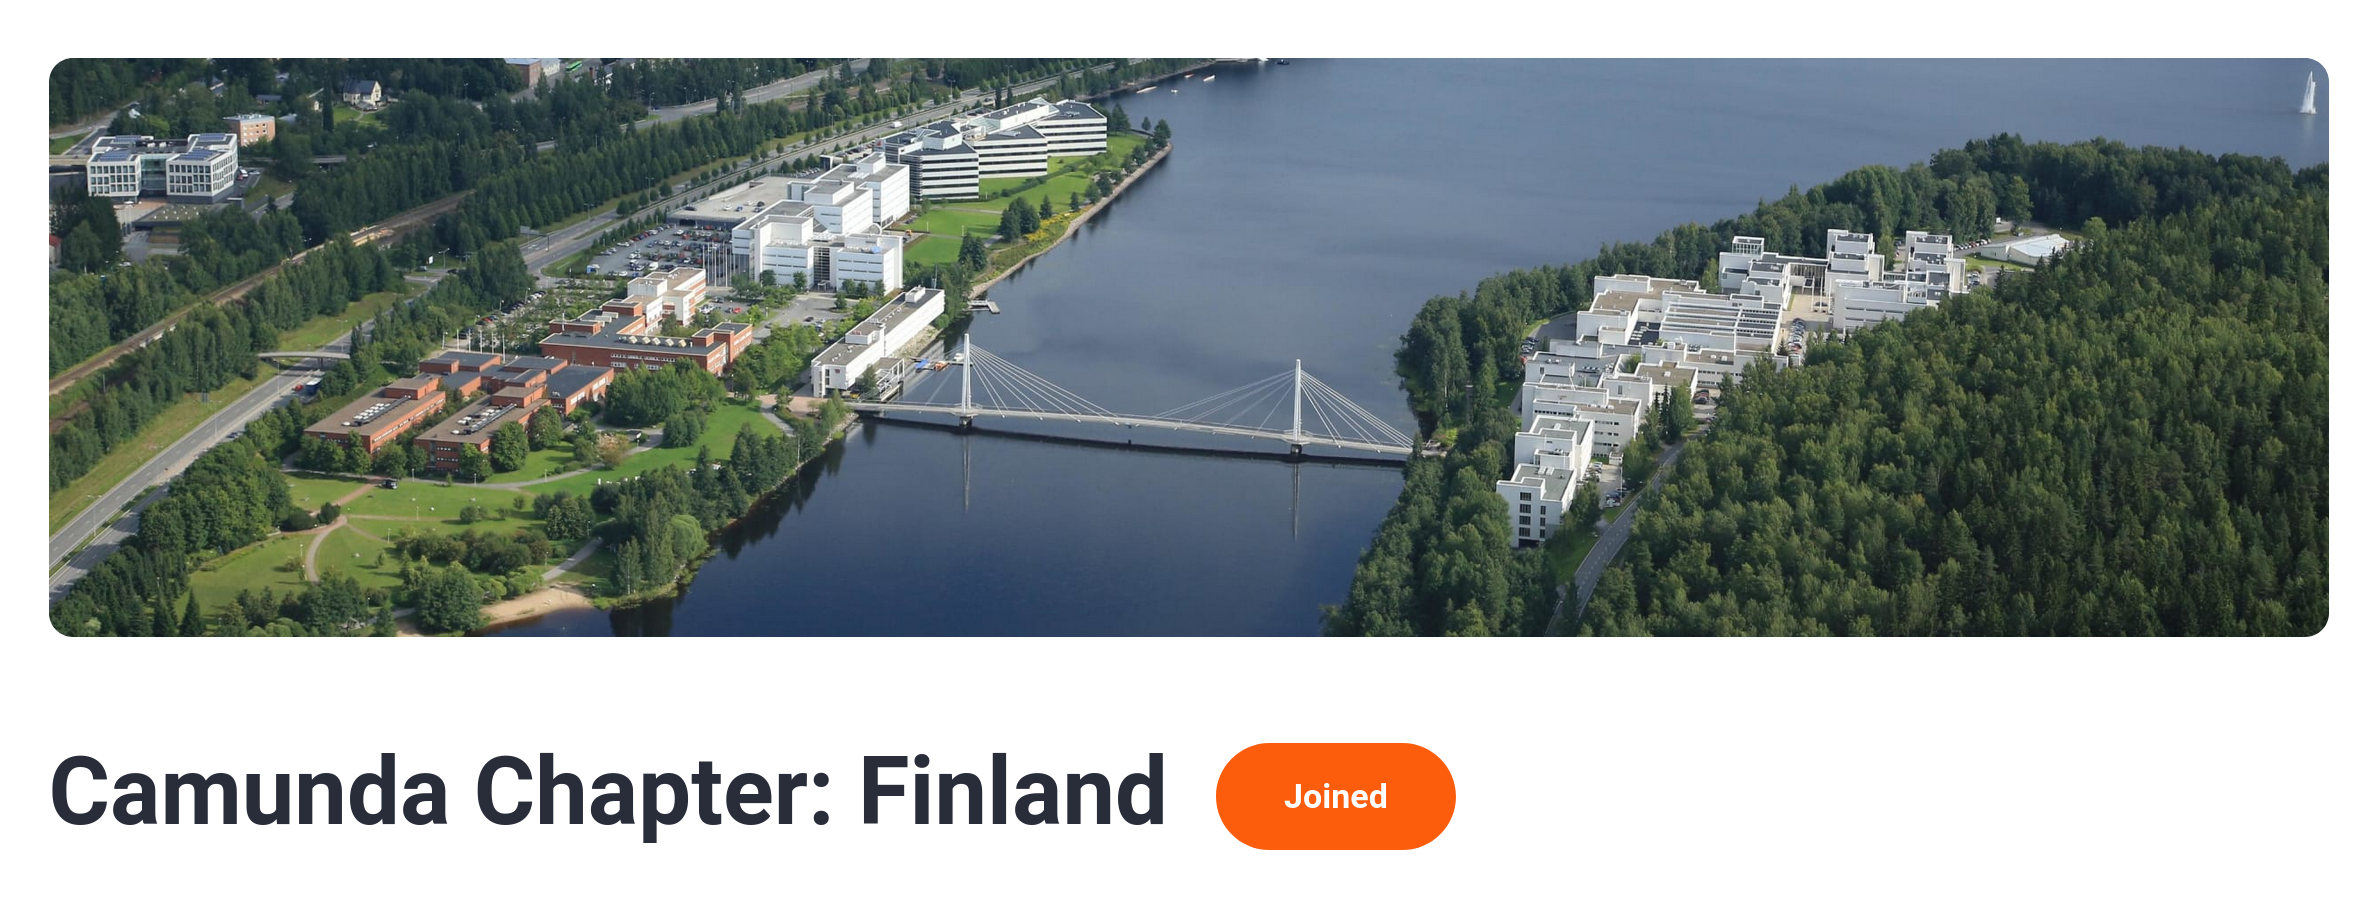
\includegraphics[width=0.875\paperwidth]{images/camunda-chapter-finland.png}
\end{frame}

\setbeamertemplate{background canvas}[default]
\begin{frame}[standout]
\begin{minipage}{0.4\textwidth}
\begin{itemize}[<+->]
  \item[] Camunda
  \item[] Chapter:
  \item[] Finland
\end{itemize}
\end{minipage}
\begin{minipage}{0.5\textwidth}
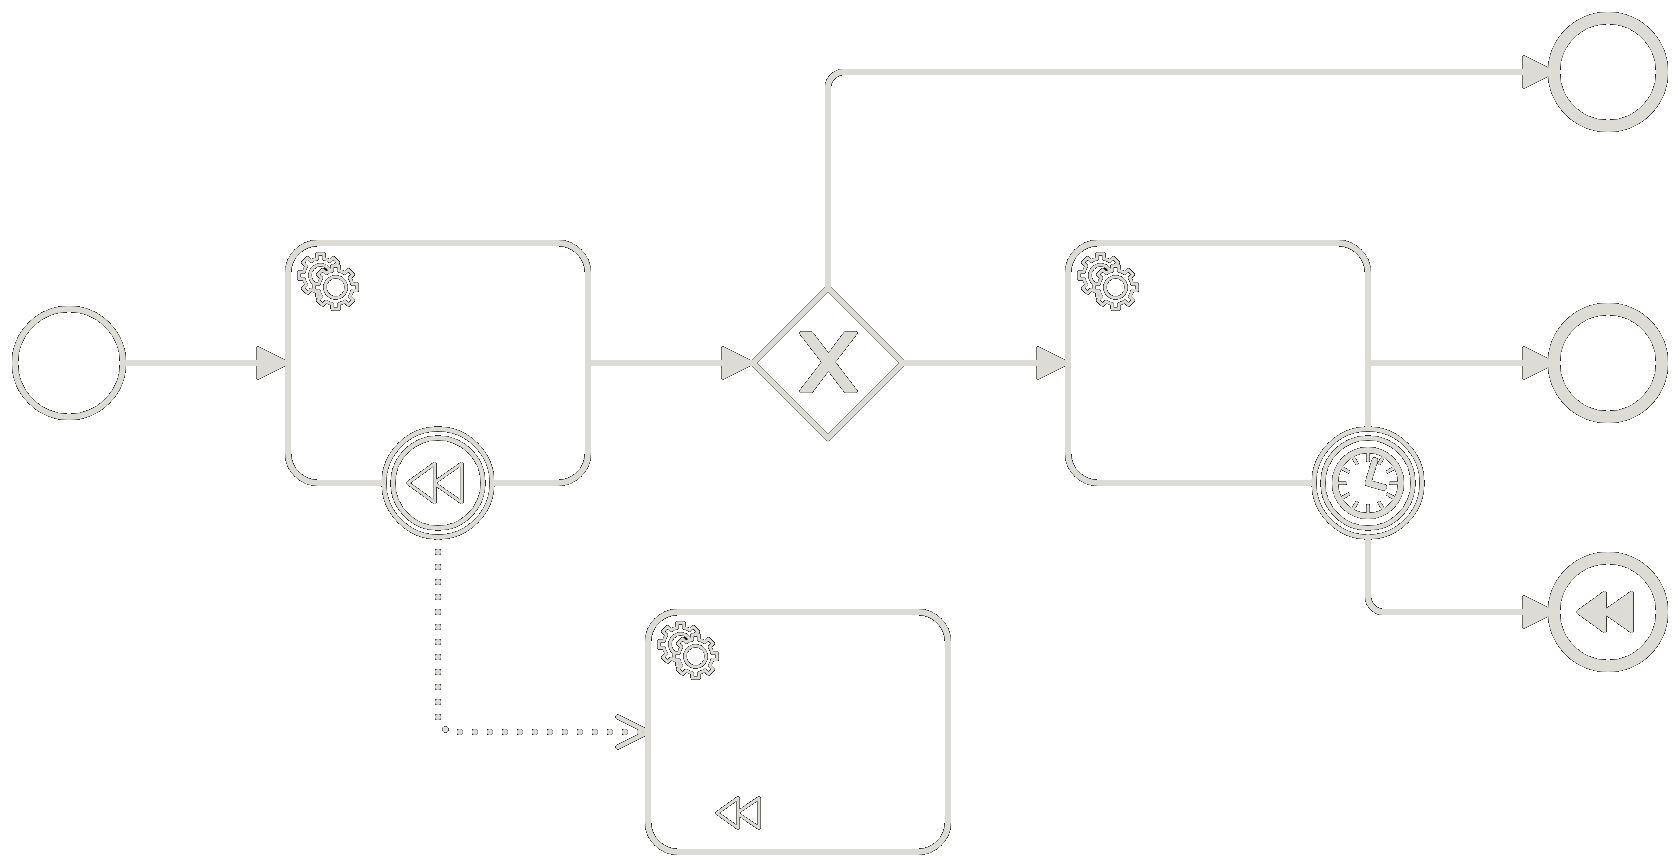
\includegraphics[width=0.8\paperwidth]{images/bpmn-example.png}
\end{minipage}
\end{frame}

%---------------------------------------------------------------------------------------

\setbeamertemplate{footline}[plain]
\setbeamertemplate{background canvas}[default]
\maketitle

%---------------------------------------------------------------------------------------

\section{Camunda Modeler}

\begin{frame}{\href{https://camunda.com/download/modeler/}{Camunda Modeler}}
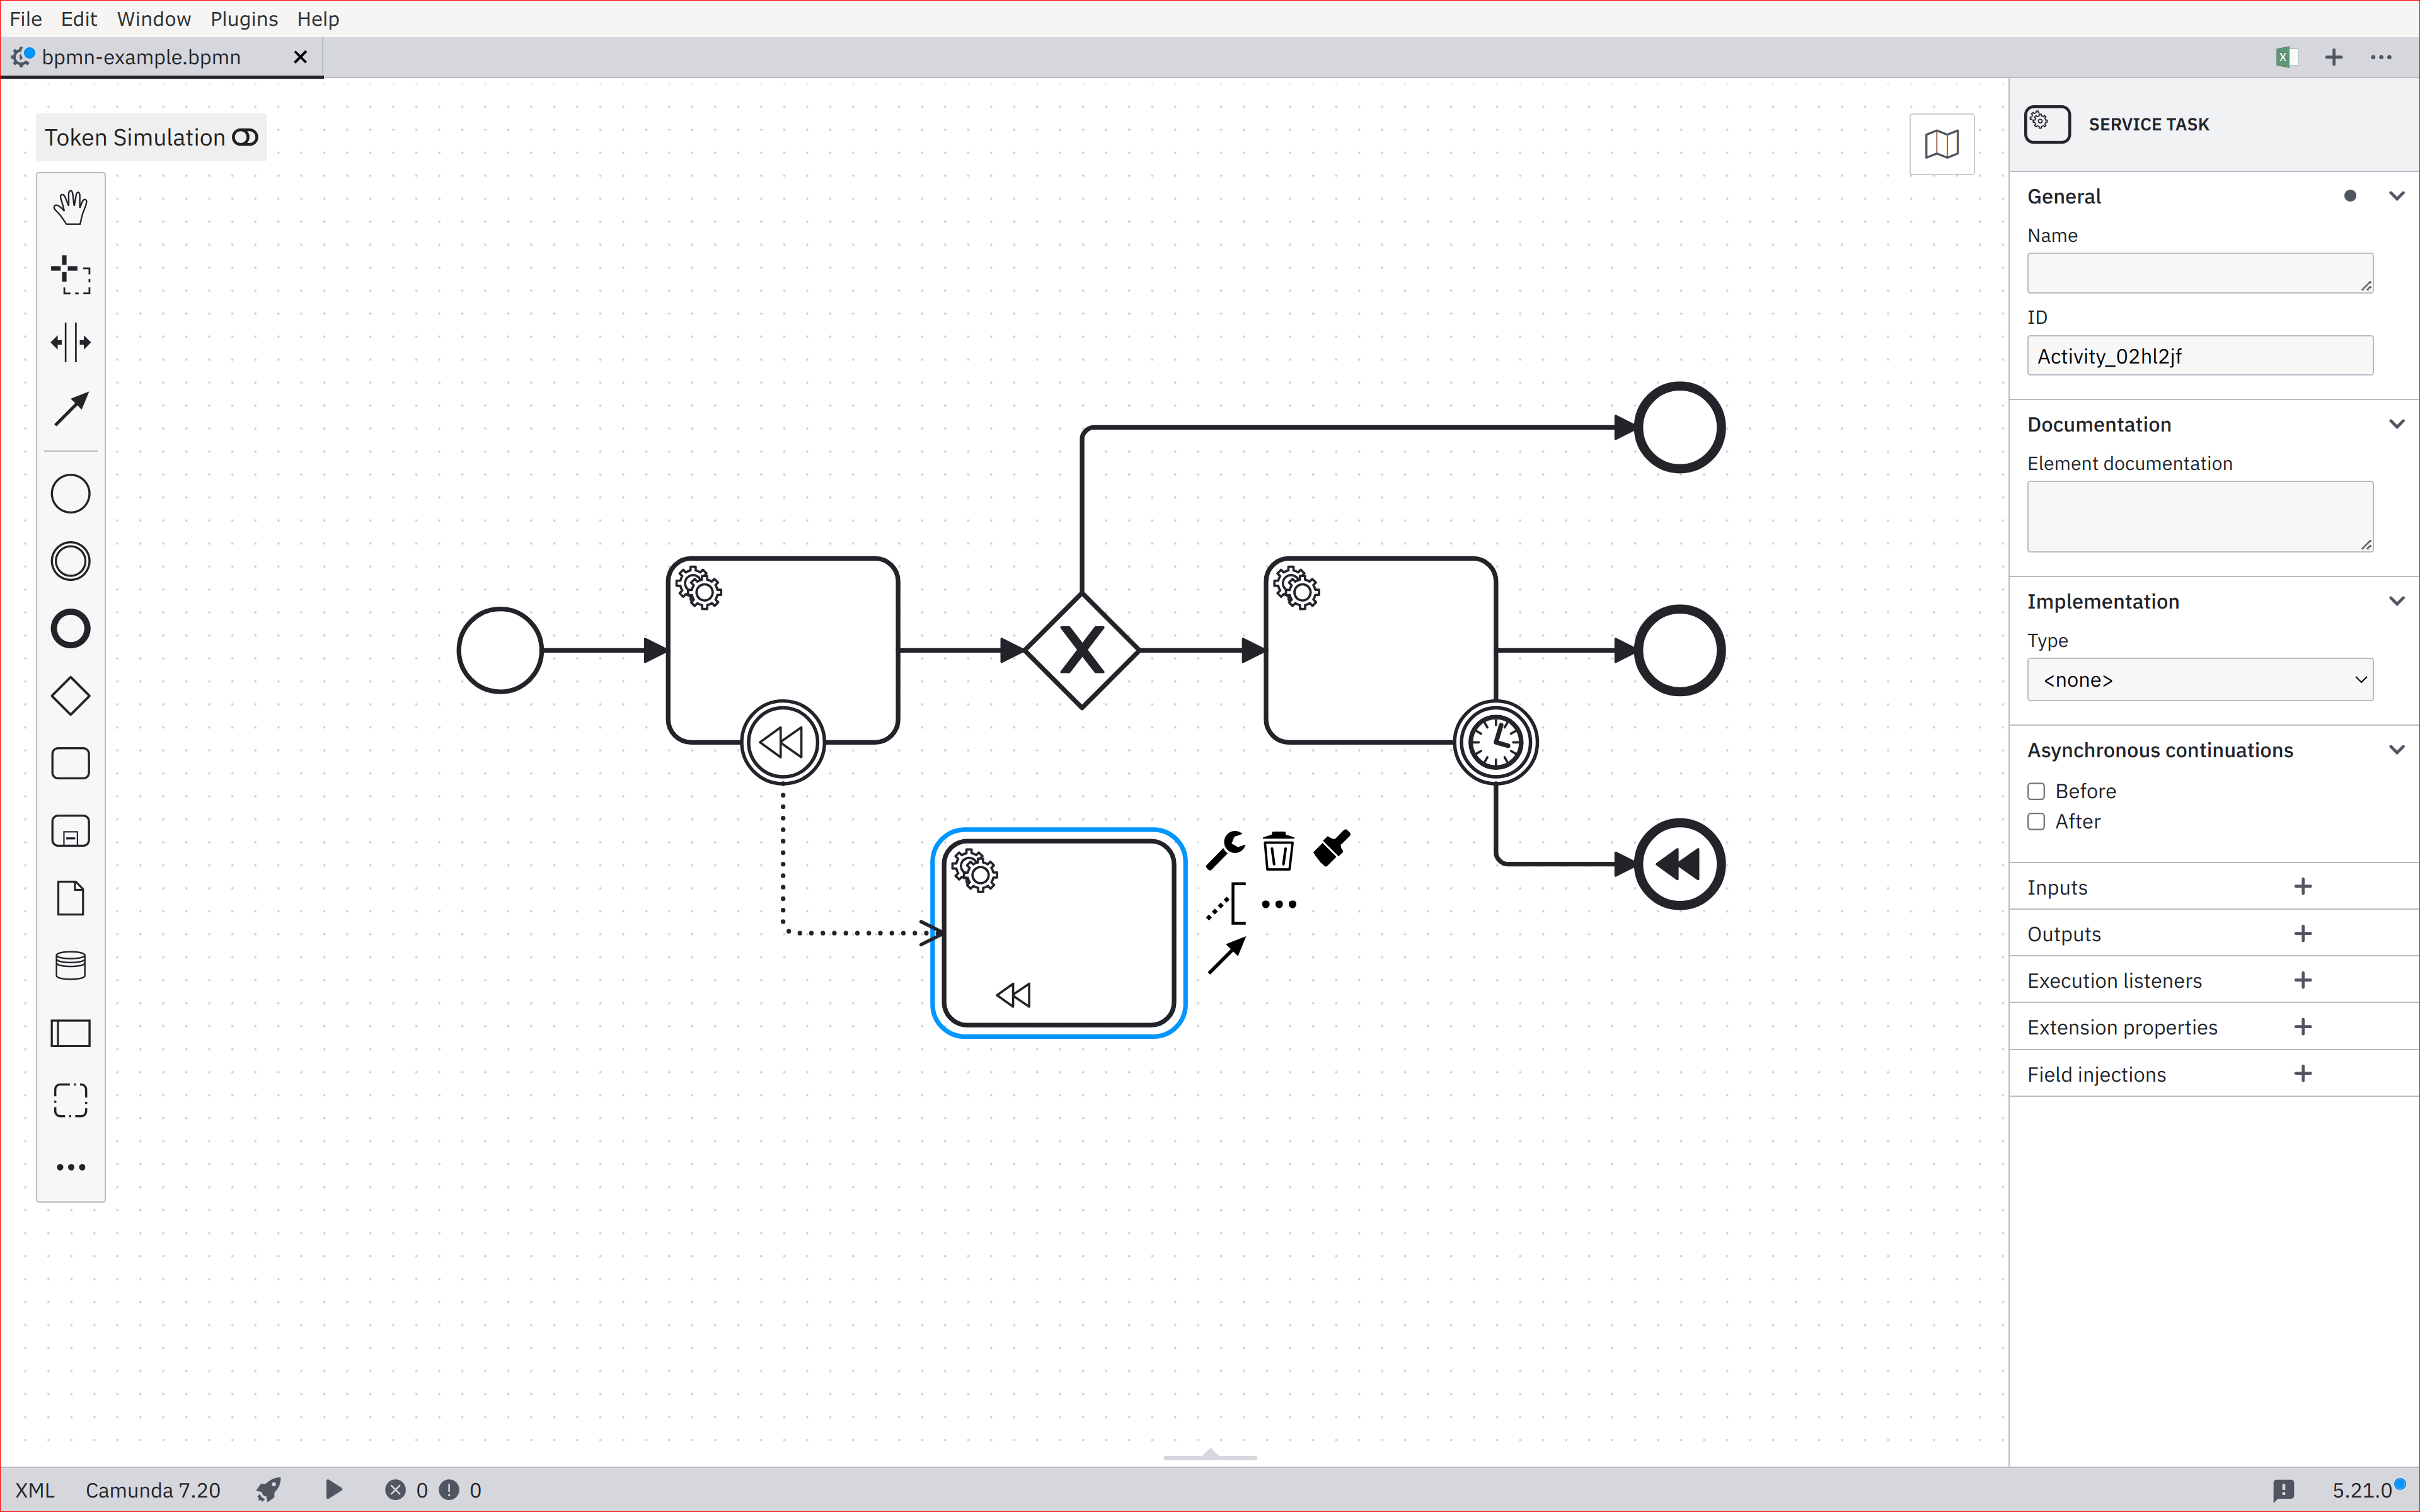
\includegraphics[width=0.8\paperwidth]{images/camunda-modeler.png}
\end{frame}

\begin{frame}{Camunda Modeler Plugins}
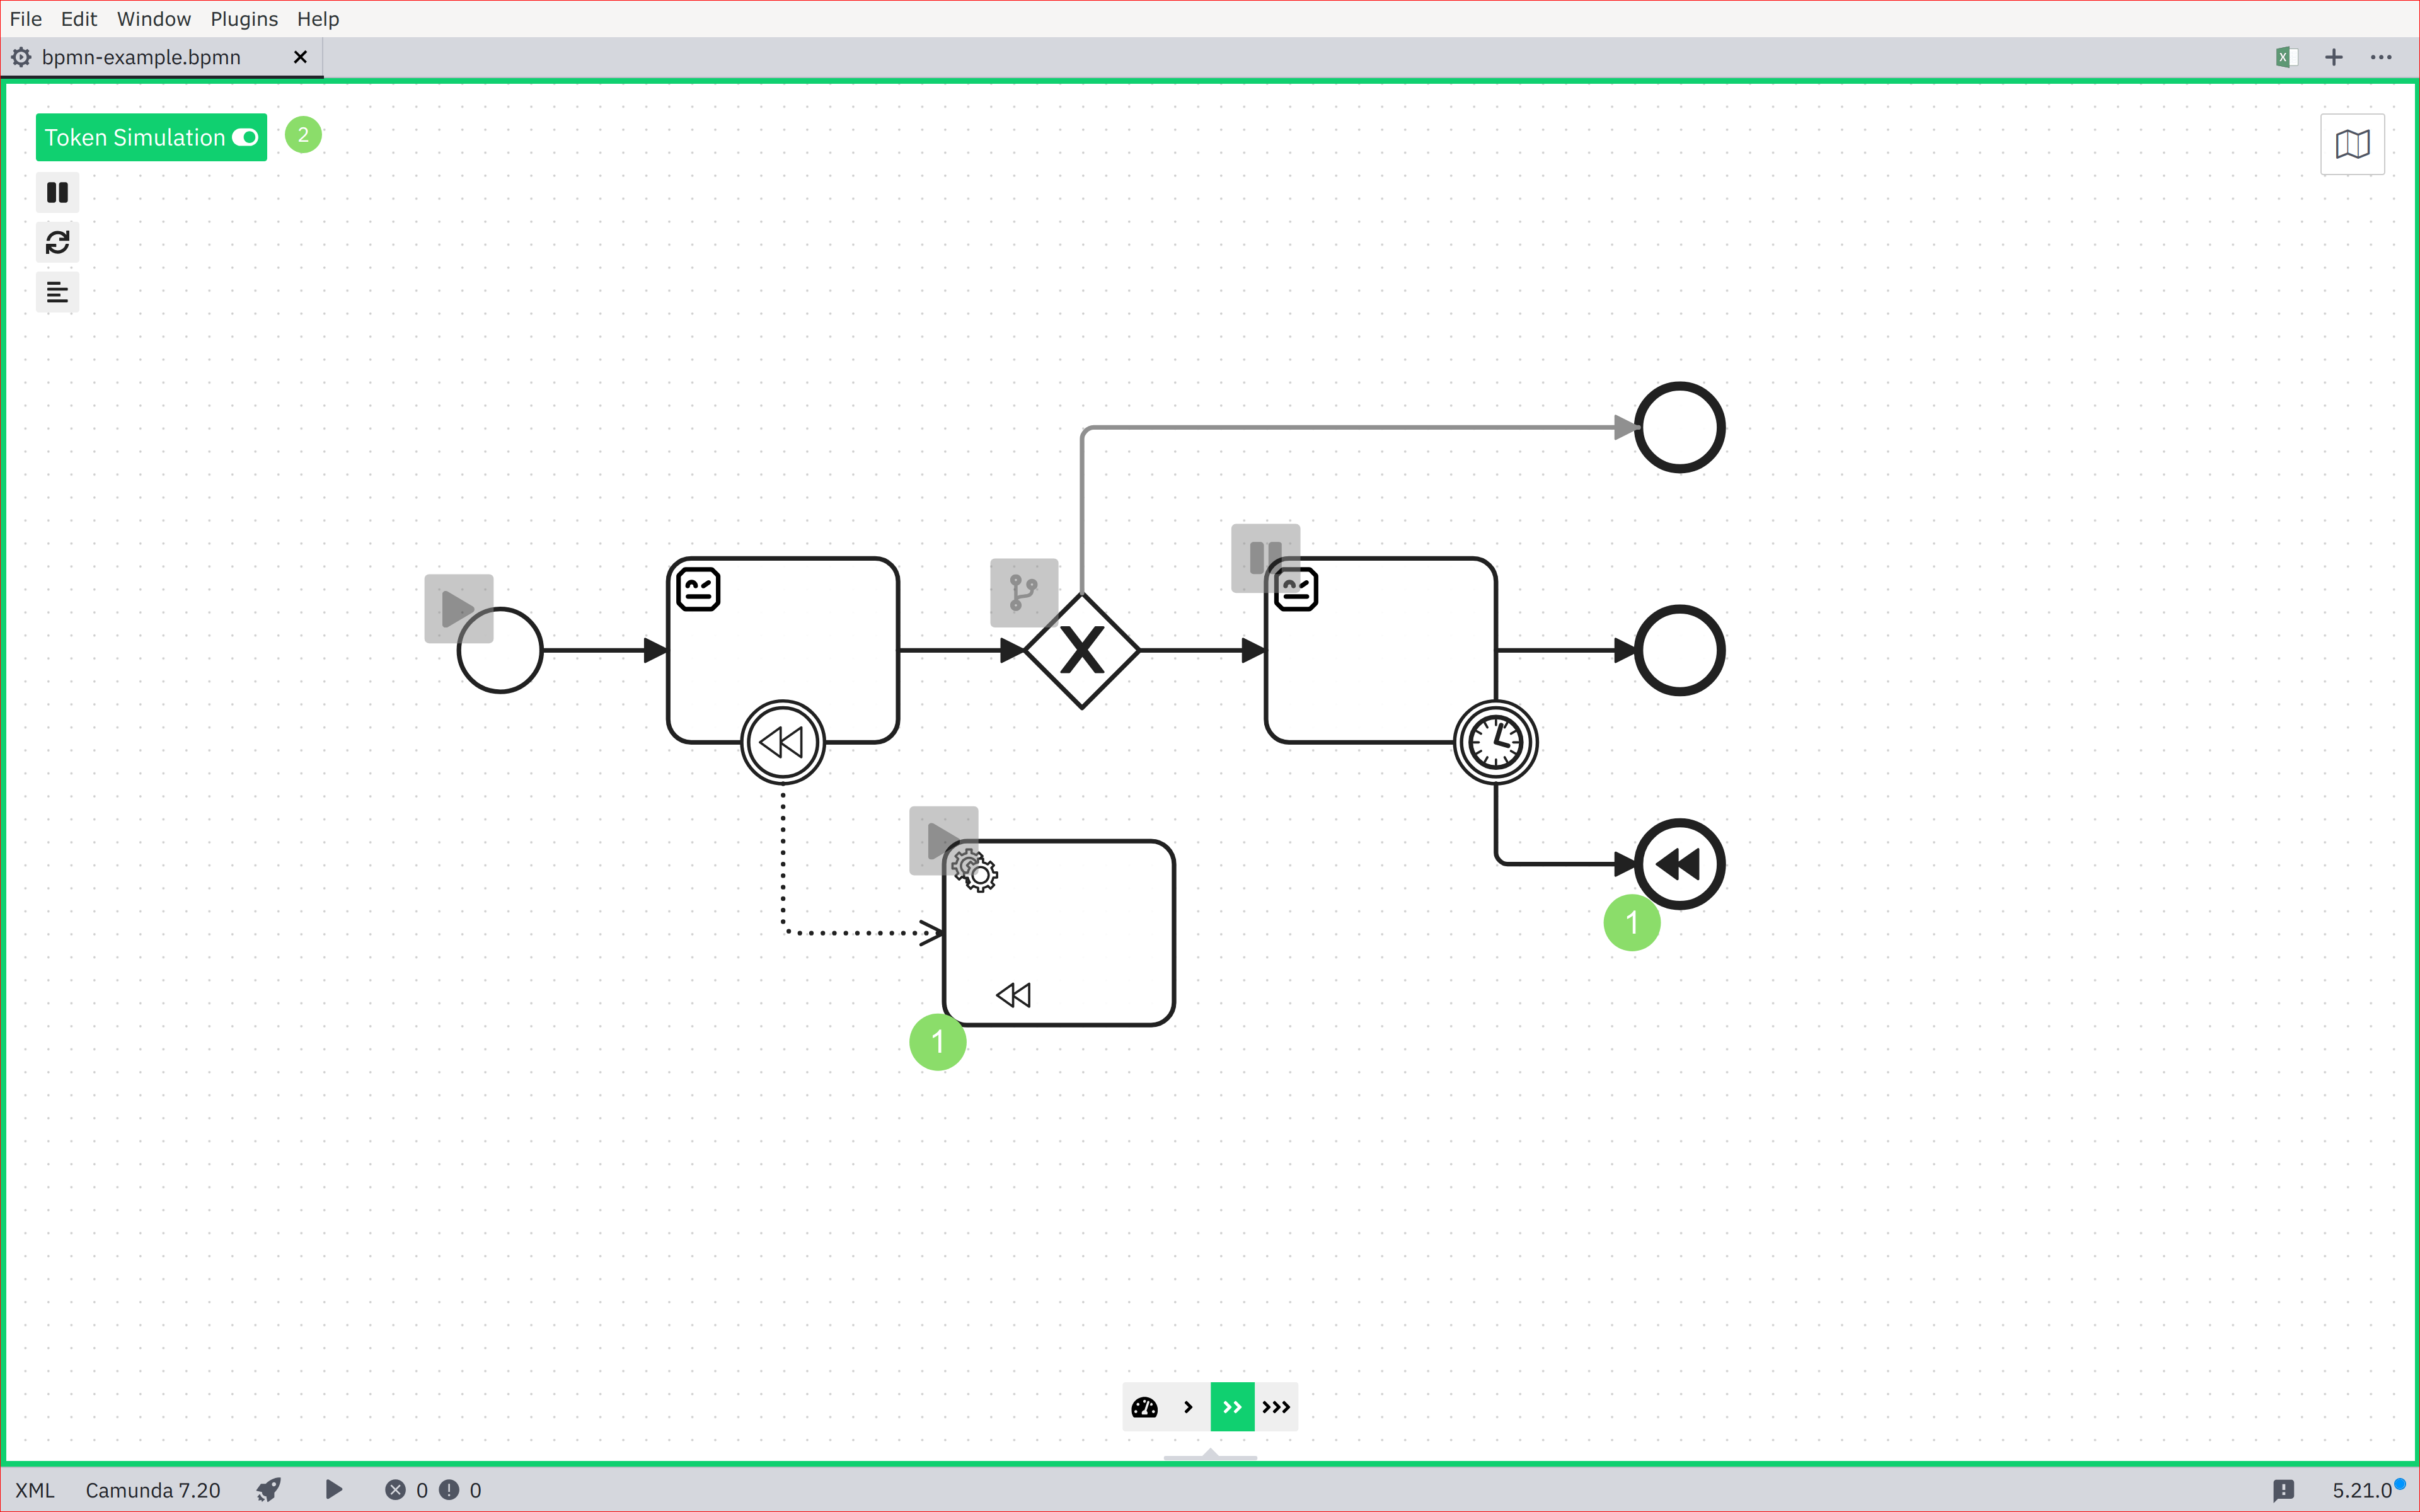
\includegraphics[width=0.8\paperwidth]{images/token-simulation.png}
\end{frame}

\begin{frame}{\href{https://camunda.com/download/modeler/}{Camunda Modeler}}
\begin{itemize}
\item License: MIT
\item Plugins:
\begin{itemize}
\item \href{https://github.com/camunda/camunda-modeler-token-simulation-plugin}{Token Simulation Plugin}
\item \href{https://github.com/camunda/camunda-modeler-plugins/tree/main/camunda-transaction-boundaries-plugin}{Transaction Boundaries Plugin}
\item \href{https://github.com/datakurre/camunda-modeler-embedded-comments-plugin}{Embedded Comments Plugin}
\item \href{https://github.com/mesoneer-ag/camunda-modeler-property-info-plugin}{Property Info Plugin}
\item \href{https://github.com/philippfromme/camunda-modeler-plugin-resize-tasks}{Resize Tasks Plugin}
\item[]
\item[] \href{https://github.com/camunda/camunda-modeler-plugins}{https://github.com/camunda/camunda-modeler-plugins}
\end{itemize}
\end{itemize}
\end{frame}


%---------------------------------------------------------------------------------------

\section{bpmn.io}

\begin{frame}{\href{https://bpmn.io/}{bpmn.io}}
\textbf{Web-based tooling for BPMN, DMN and Forms}
\par
\vspace{0.5cm}
\par
\begin{minipage}{0.5\textwidth}
\begin{itemize}[<+->]
    \item \href{http://demo.bpmn.io/}{bpmn-js}
    \item \href{http://demo.bpmn.io/dmn}{dmn-js}
    \item \href{http://demo.bpmn.io/form}{form-js}
    \item \href{https://nikku.github.io/feel-playground/}{nikku/feelin}
    \item \href{http://demo.bpmn.io/cmmn}{cmmn-js}
\end{itemize}
\end{minipage}
\begin{minipage}{0.45\textwidth}
    \begin{tikzpicture}[remember picture, overlay]
        \node<1> at ([yshift=-1cm, xshift=1cm]current page.center) {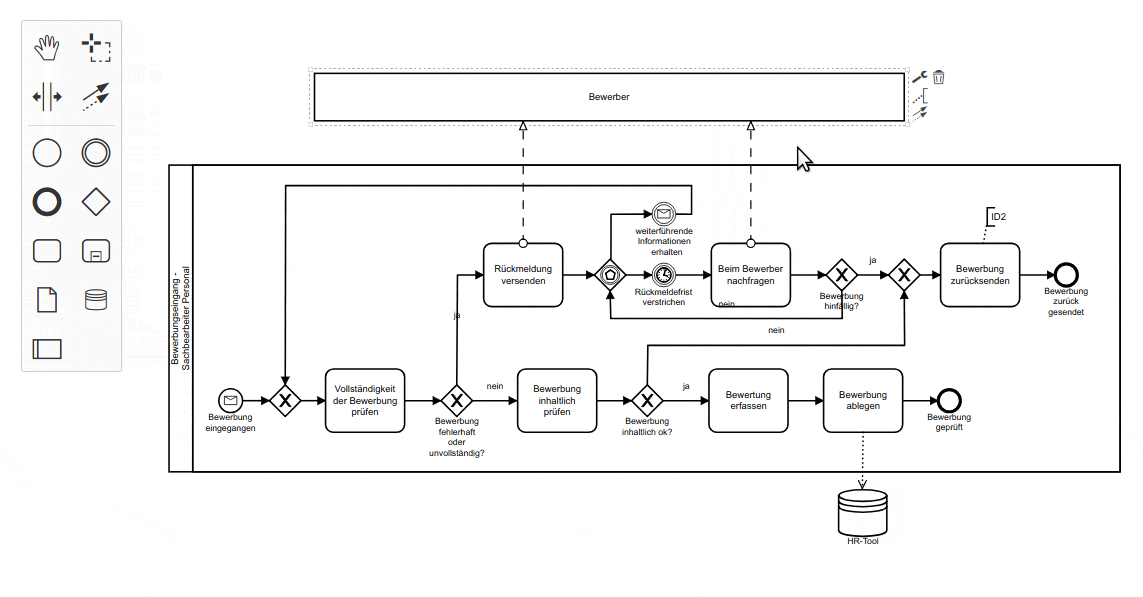
\includegraphics[width=1\textwidth]{images/bpmn-js.png}};
        \node<2> at ([yshift=-1cm, xshift=1cm]current page.center) {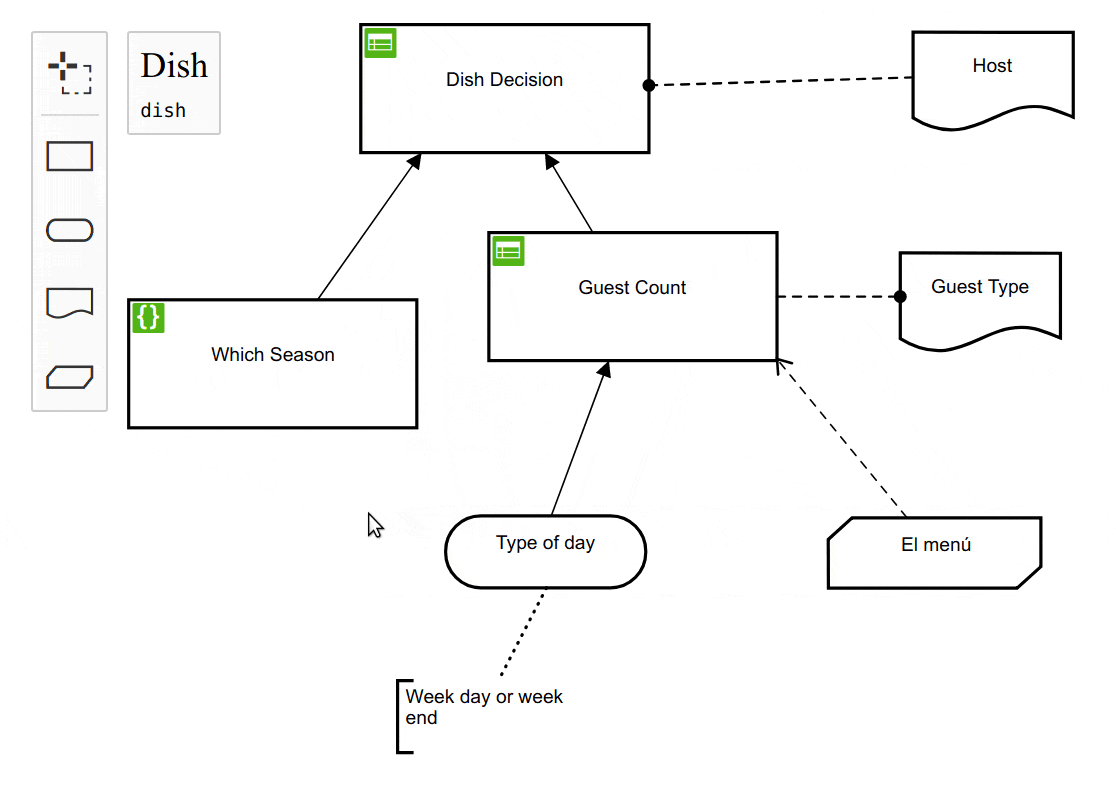
\includegraphics[width=1\textwidth]{images/dmn-js.png}};
        \node<3> at ([yshift=-1cm, xshift=1cm]current page.center) {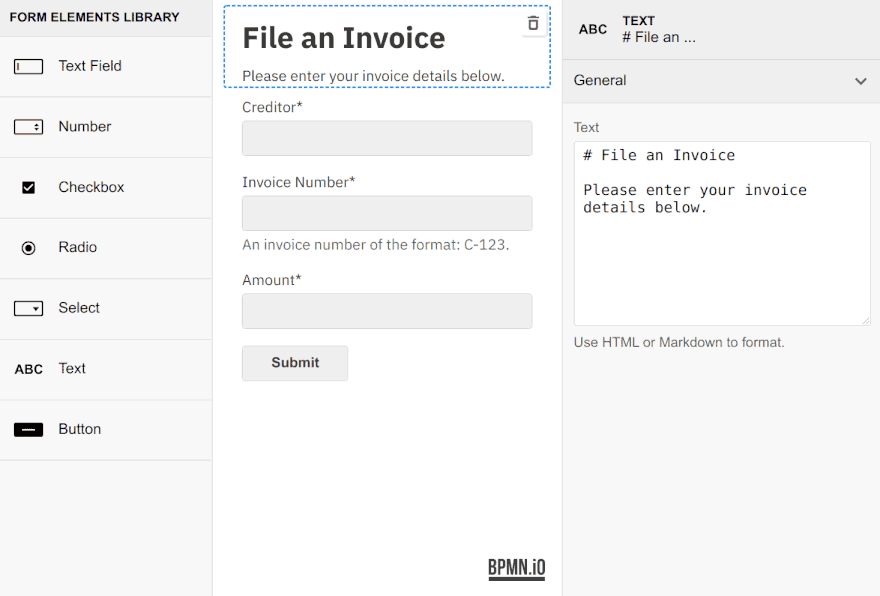
\includegraphics[width=1\textwidth]{images/form-js.png}};
        \node<4> at ([yshift=-1cm, xshift=1cm]current page.center) {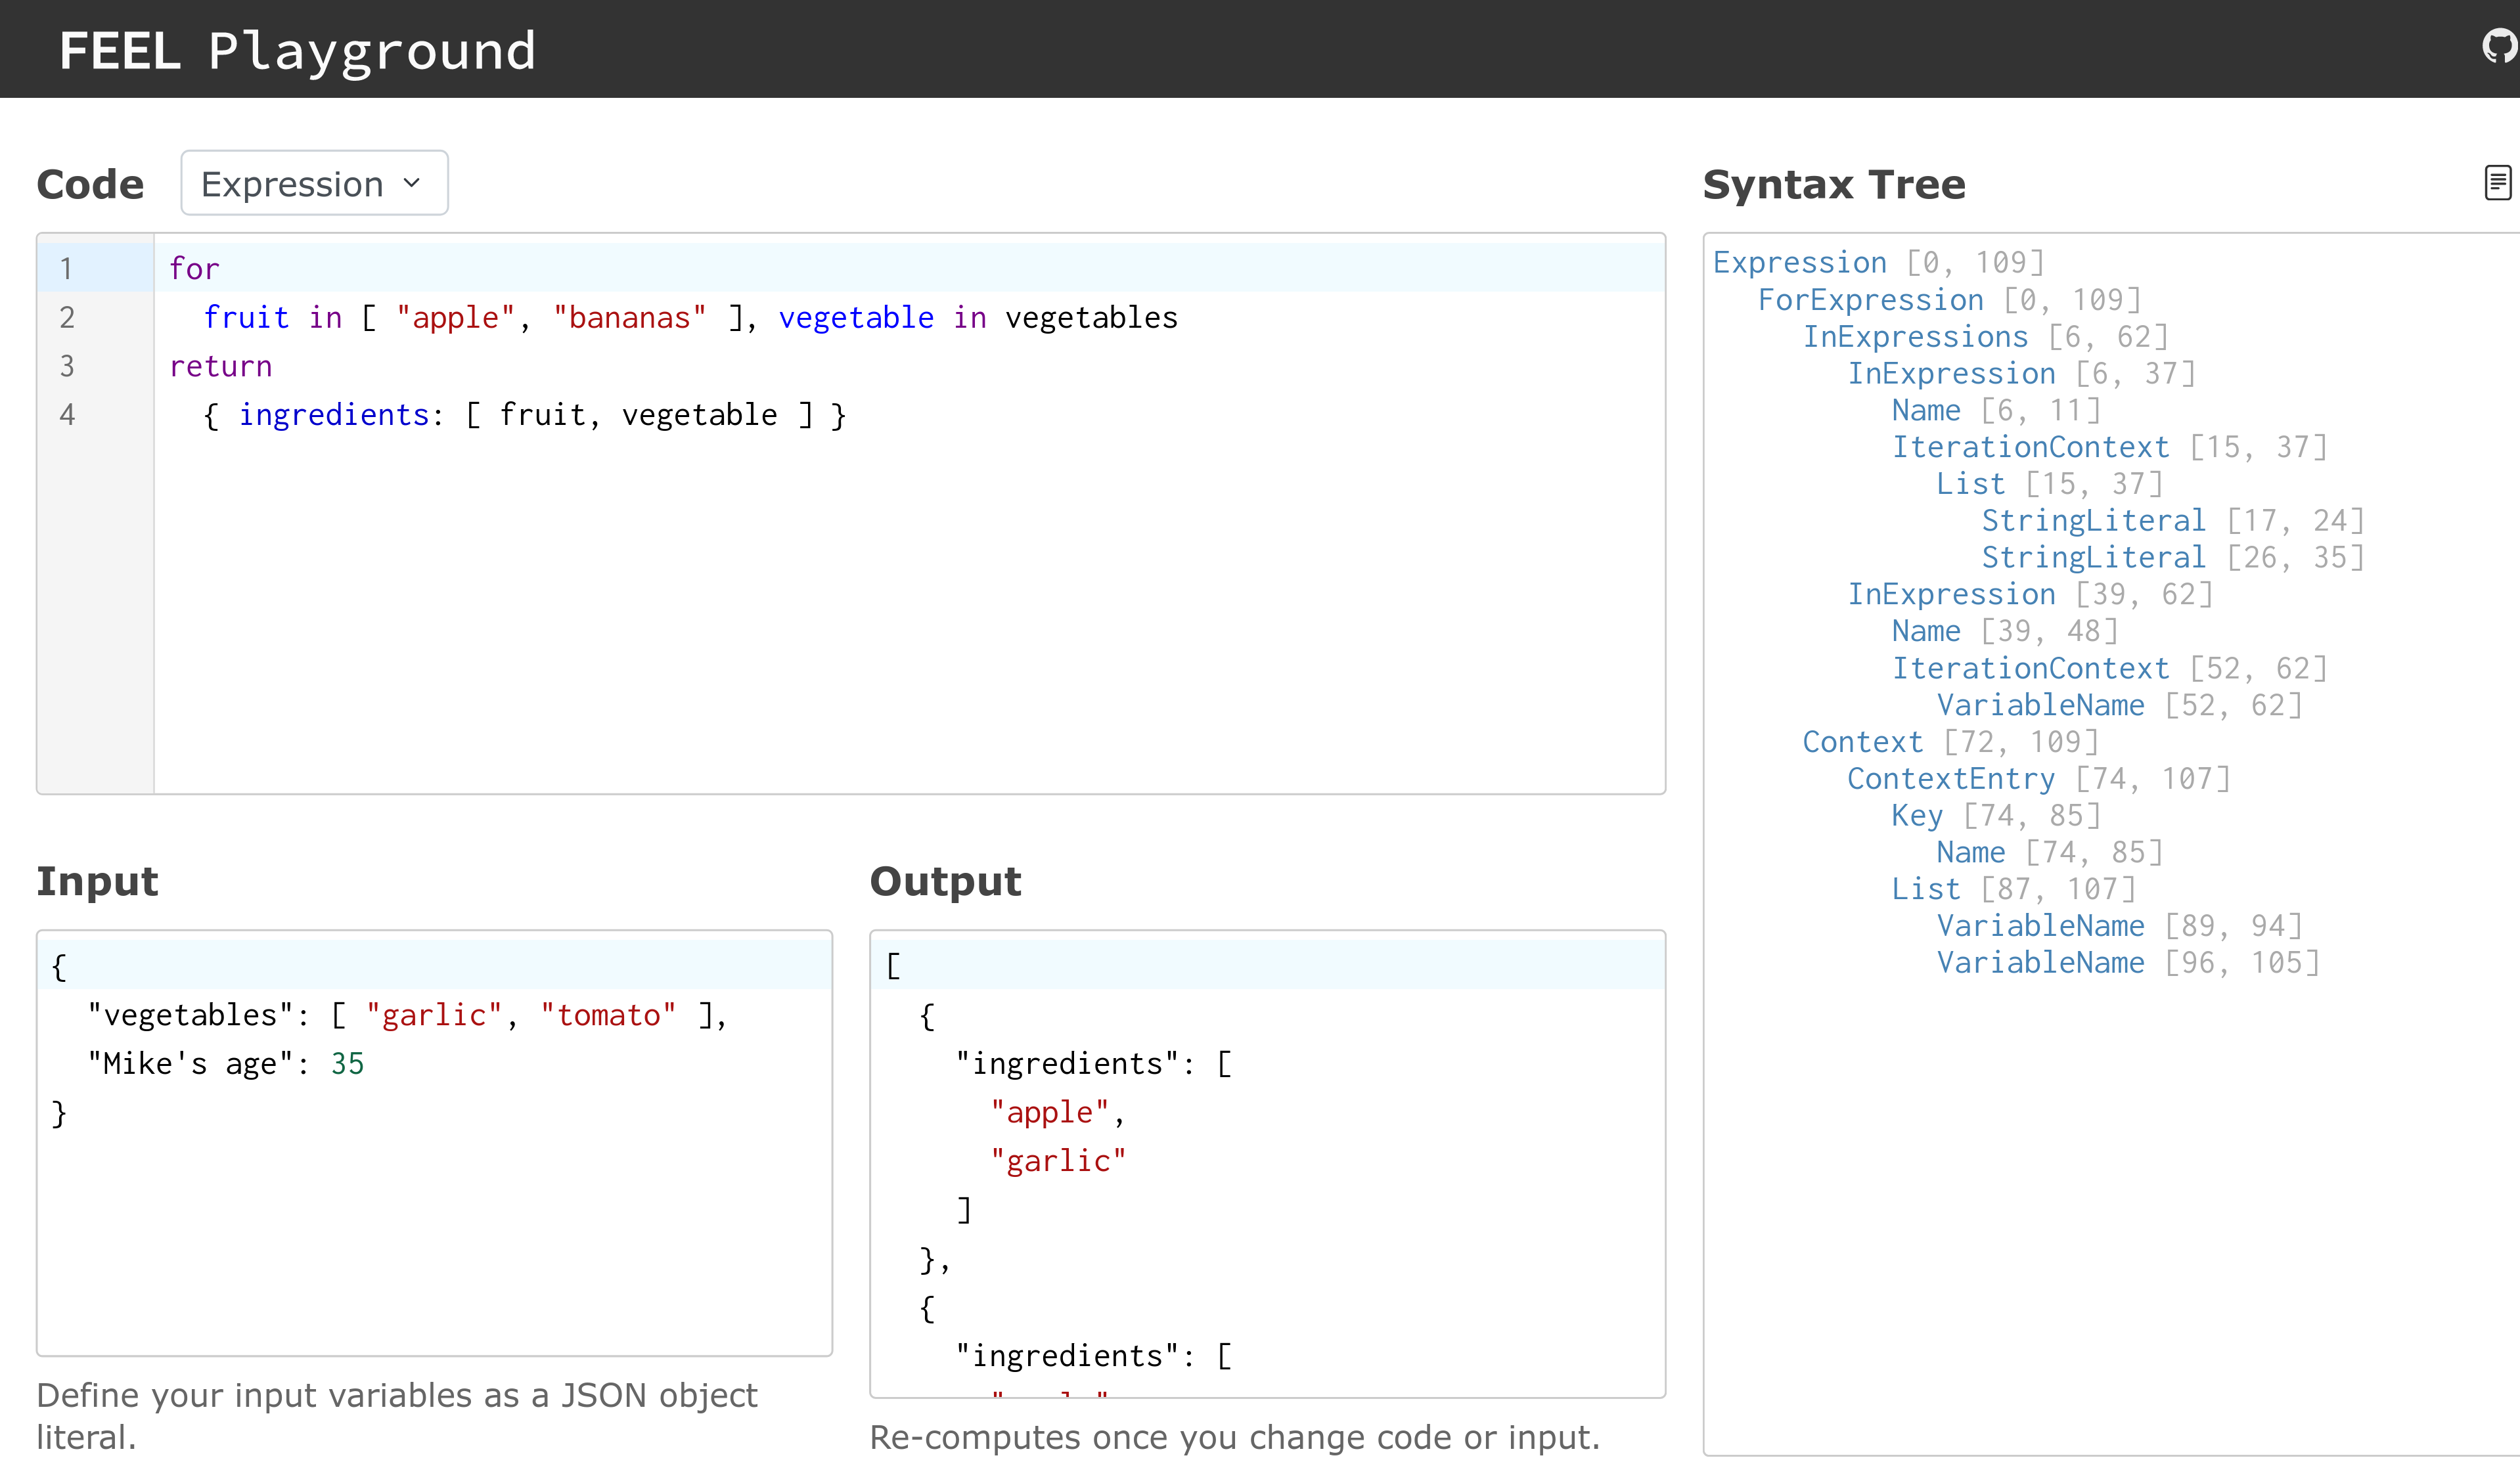
\includegraphics[width=1\textwidth]{images/feelin-playground.png}};
        \node<5> at ([yshift=-1cm, xshift=1cm]current page.center) {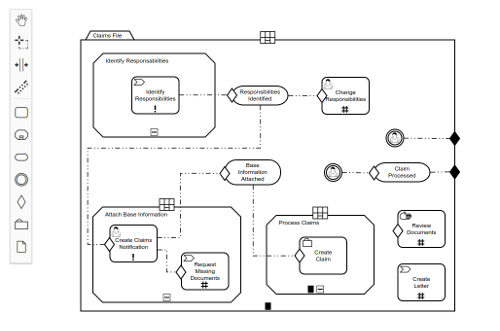
\includegraphics[width=1\textwidth]{images/cmmn-js.png}};
    \end{tikzpicture}
\end{minipage}
\end{frame}

\begin{frame}{bpmn.io + JupyterLab}
\textbf{BPMN, DMN and Forms in Jupyter notebooks}
\par
\vspace{0.5cm}
\par
\begin{minipage}{0.5\textwidth}
\begin{itemize}
    \item<1->  \href{https://github.com/datakurre/jupyterlab-bpmn}{jupyterlab-bpmn}
    \item<2-> \href{https://github.com/datakurre/jupyterlab-dmn}{jupyterlab-dmn}
    \item<3-> \href{https://github.com/datakurre/jupyterlab-form-js}{jupyterlab-form-js}
    \item[]
    \item[]
\end{itemize}
\end{minipage}
\begin{minipage}{0.45\textwidth}
    \begin{tikzpicture}[remember picture, overlay]
        \node<1> at ([yshift=-1cm, xshift=1cm]current page.center) {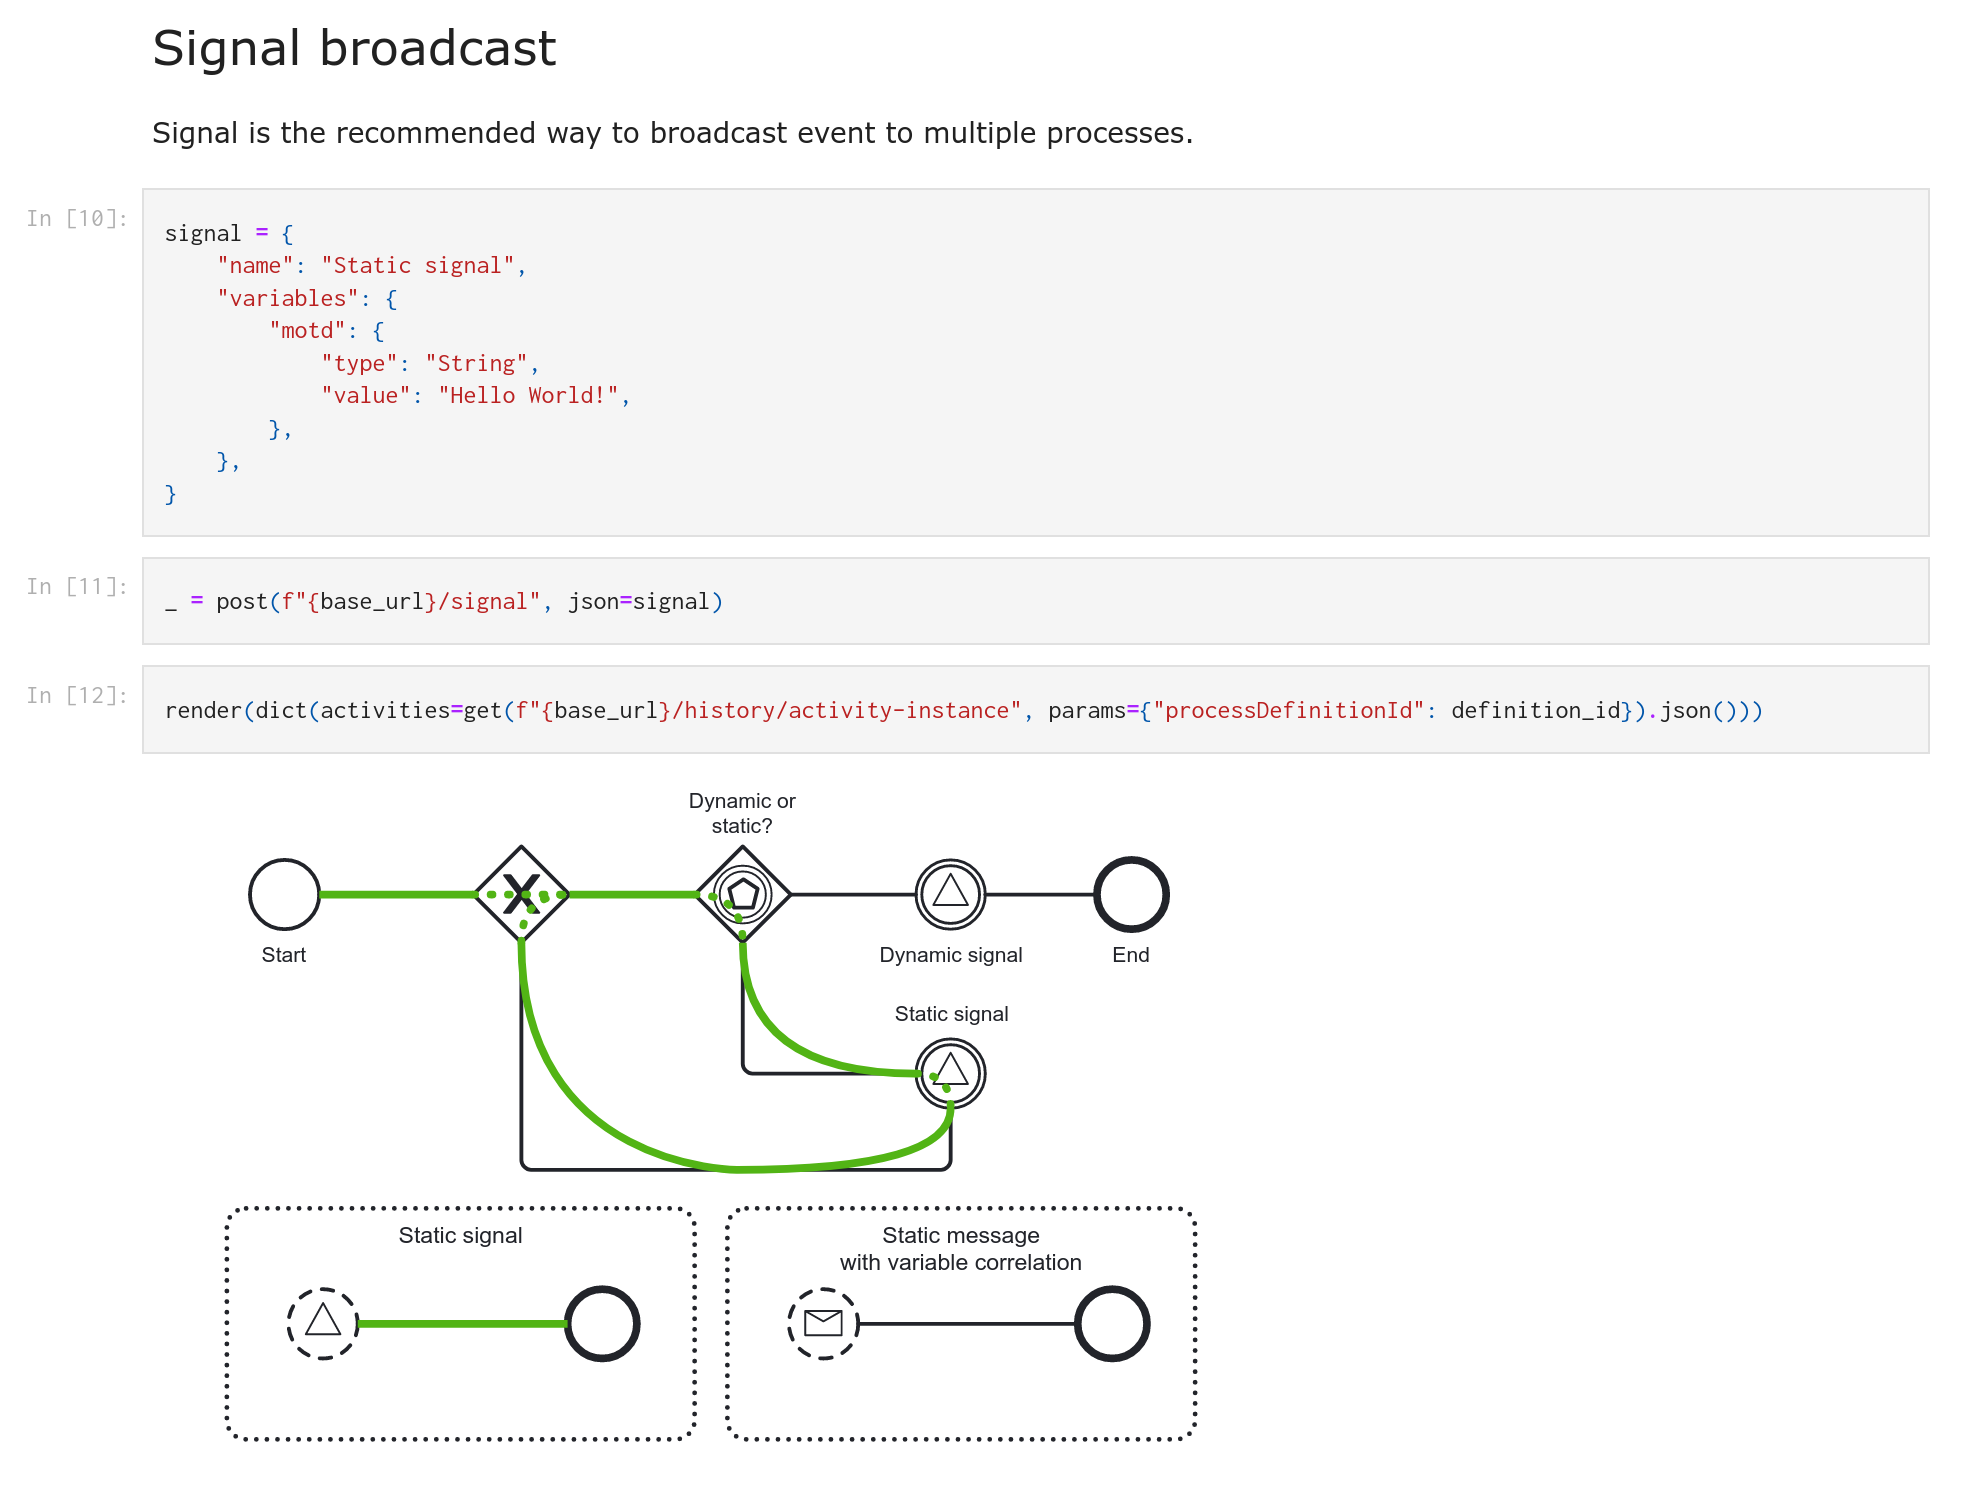
\includegraphics[width=1\textwidth]{images/jupyterlab-bpmn.png}};
        \node<3> at ([yshift=-1cm, xshift=1cm]current page.center) {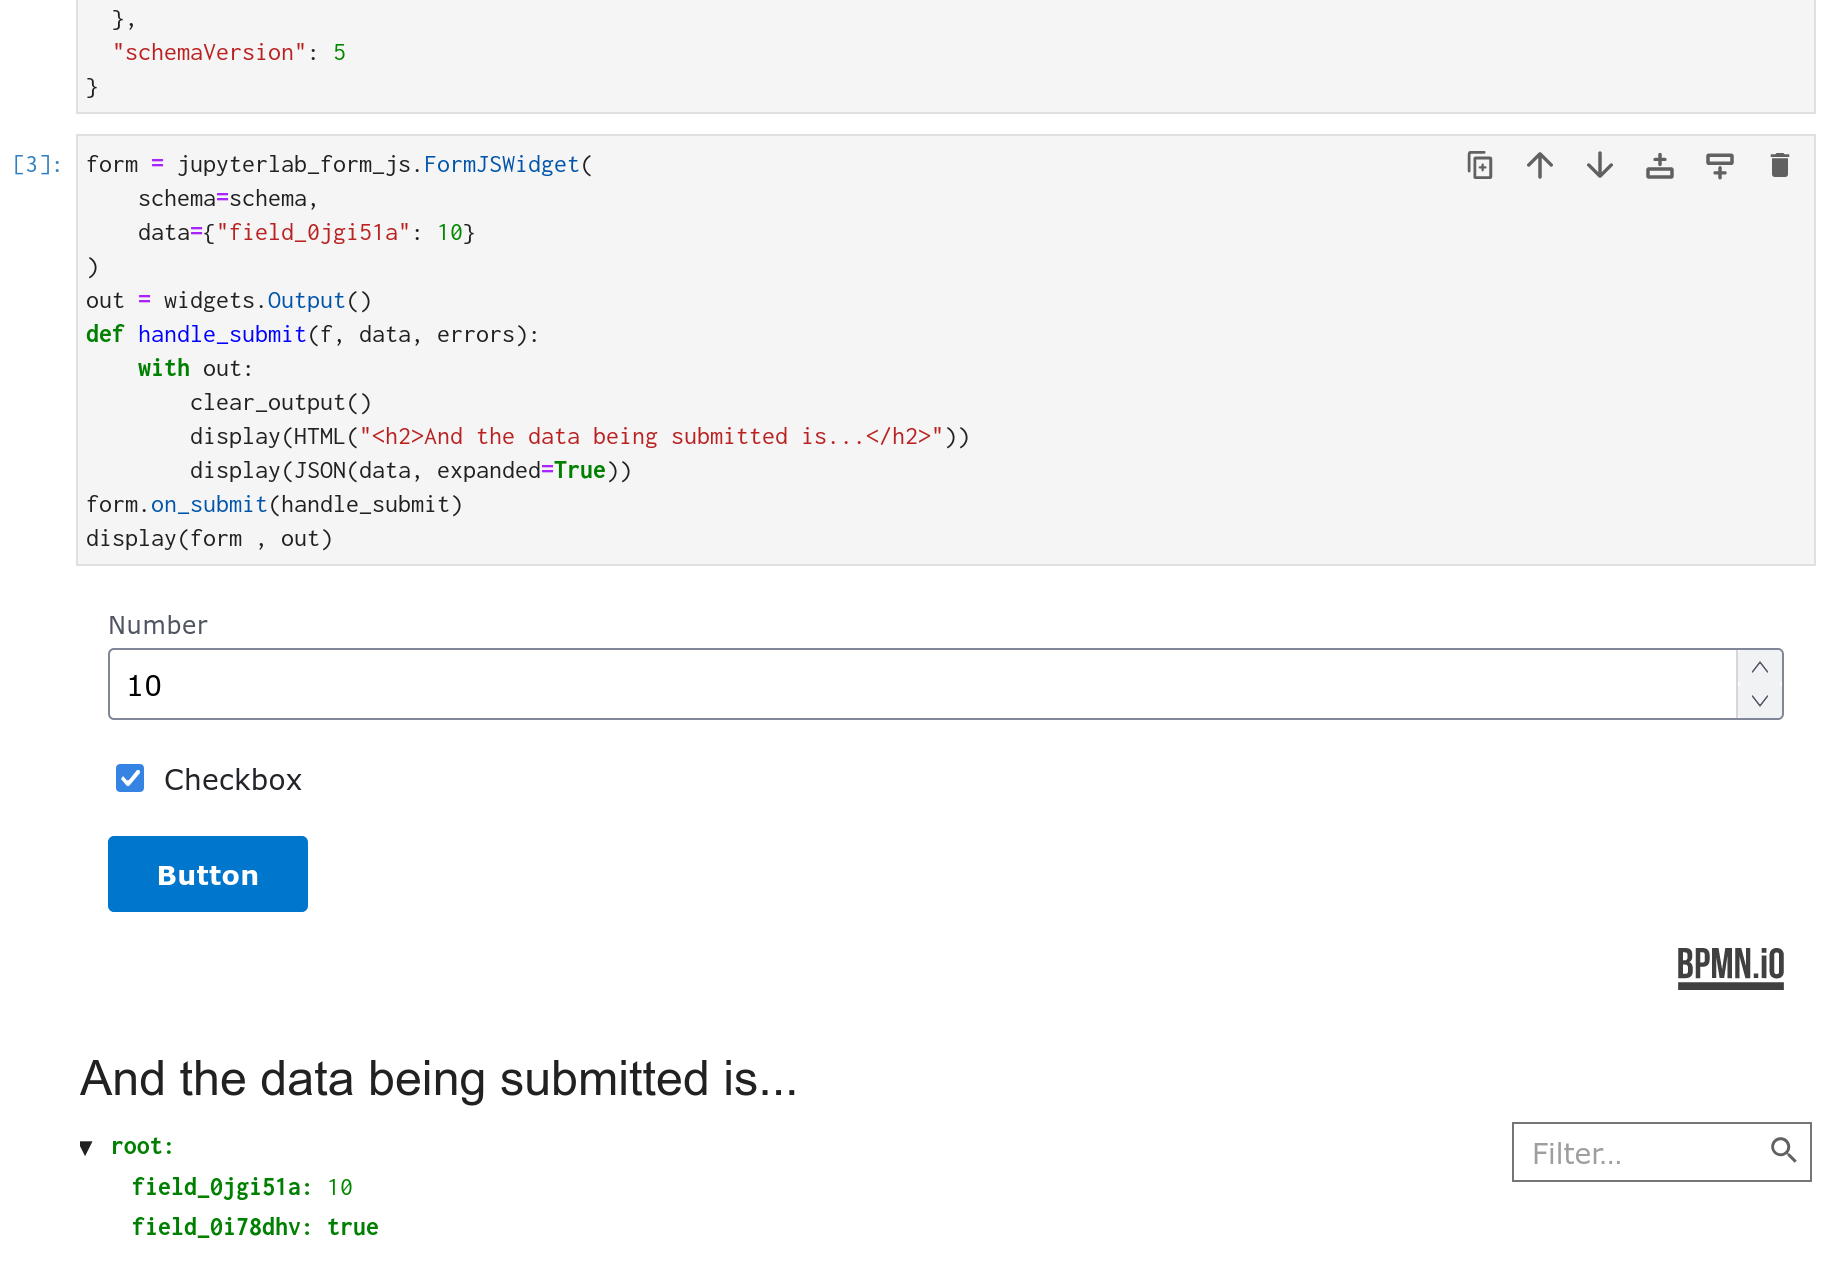
\includegraphics[width=1\textwidth]{images/jupyterlab-form-js.png}};
    \end{tikzpicture}
\end{minipage}
\end{frame}

\begin{frame}{Sphinx documentation}
\centering
\href{https://datakurre.github.io/automation-playground}{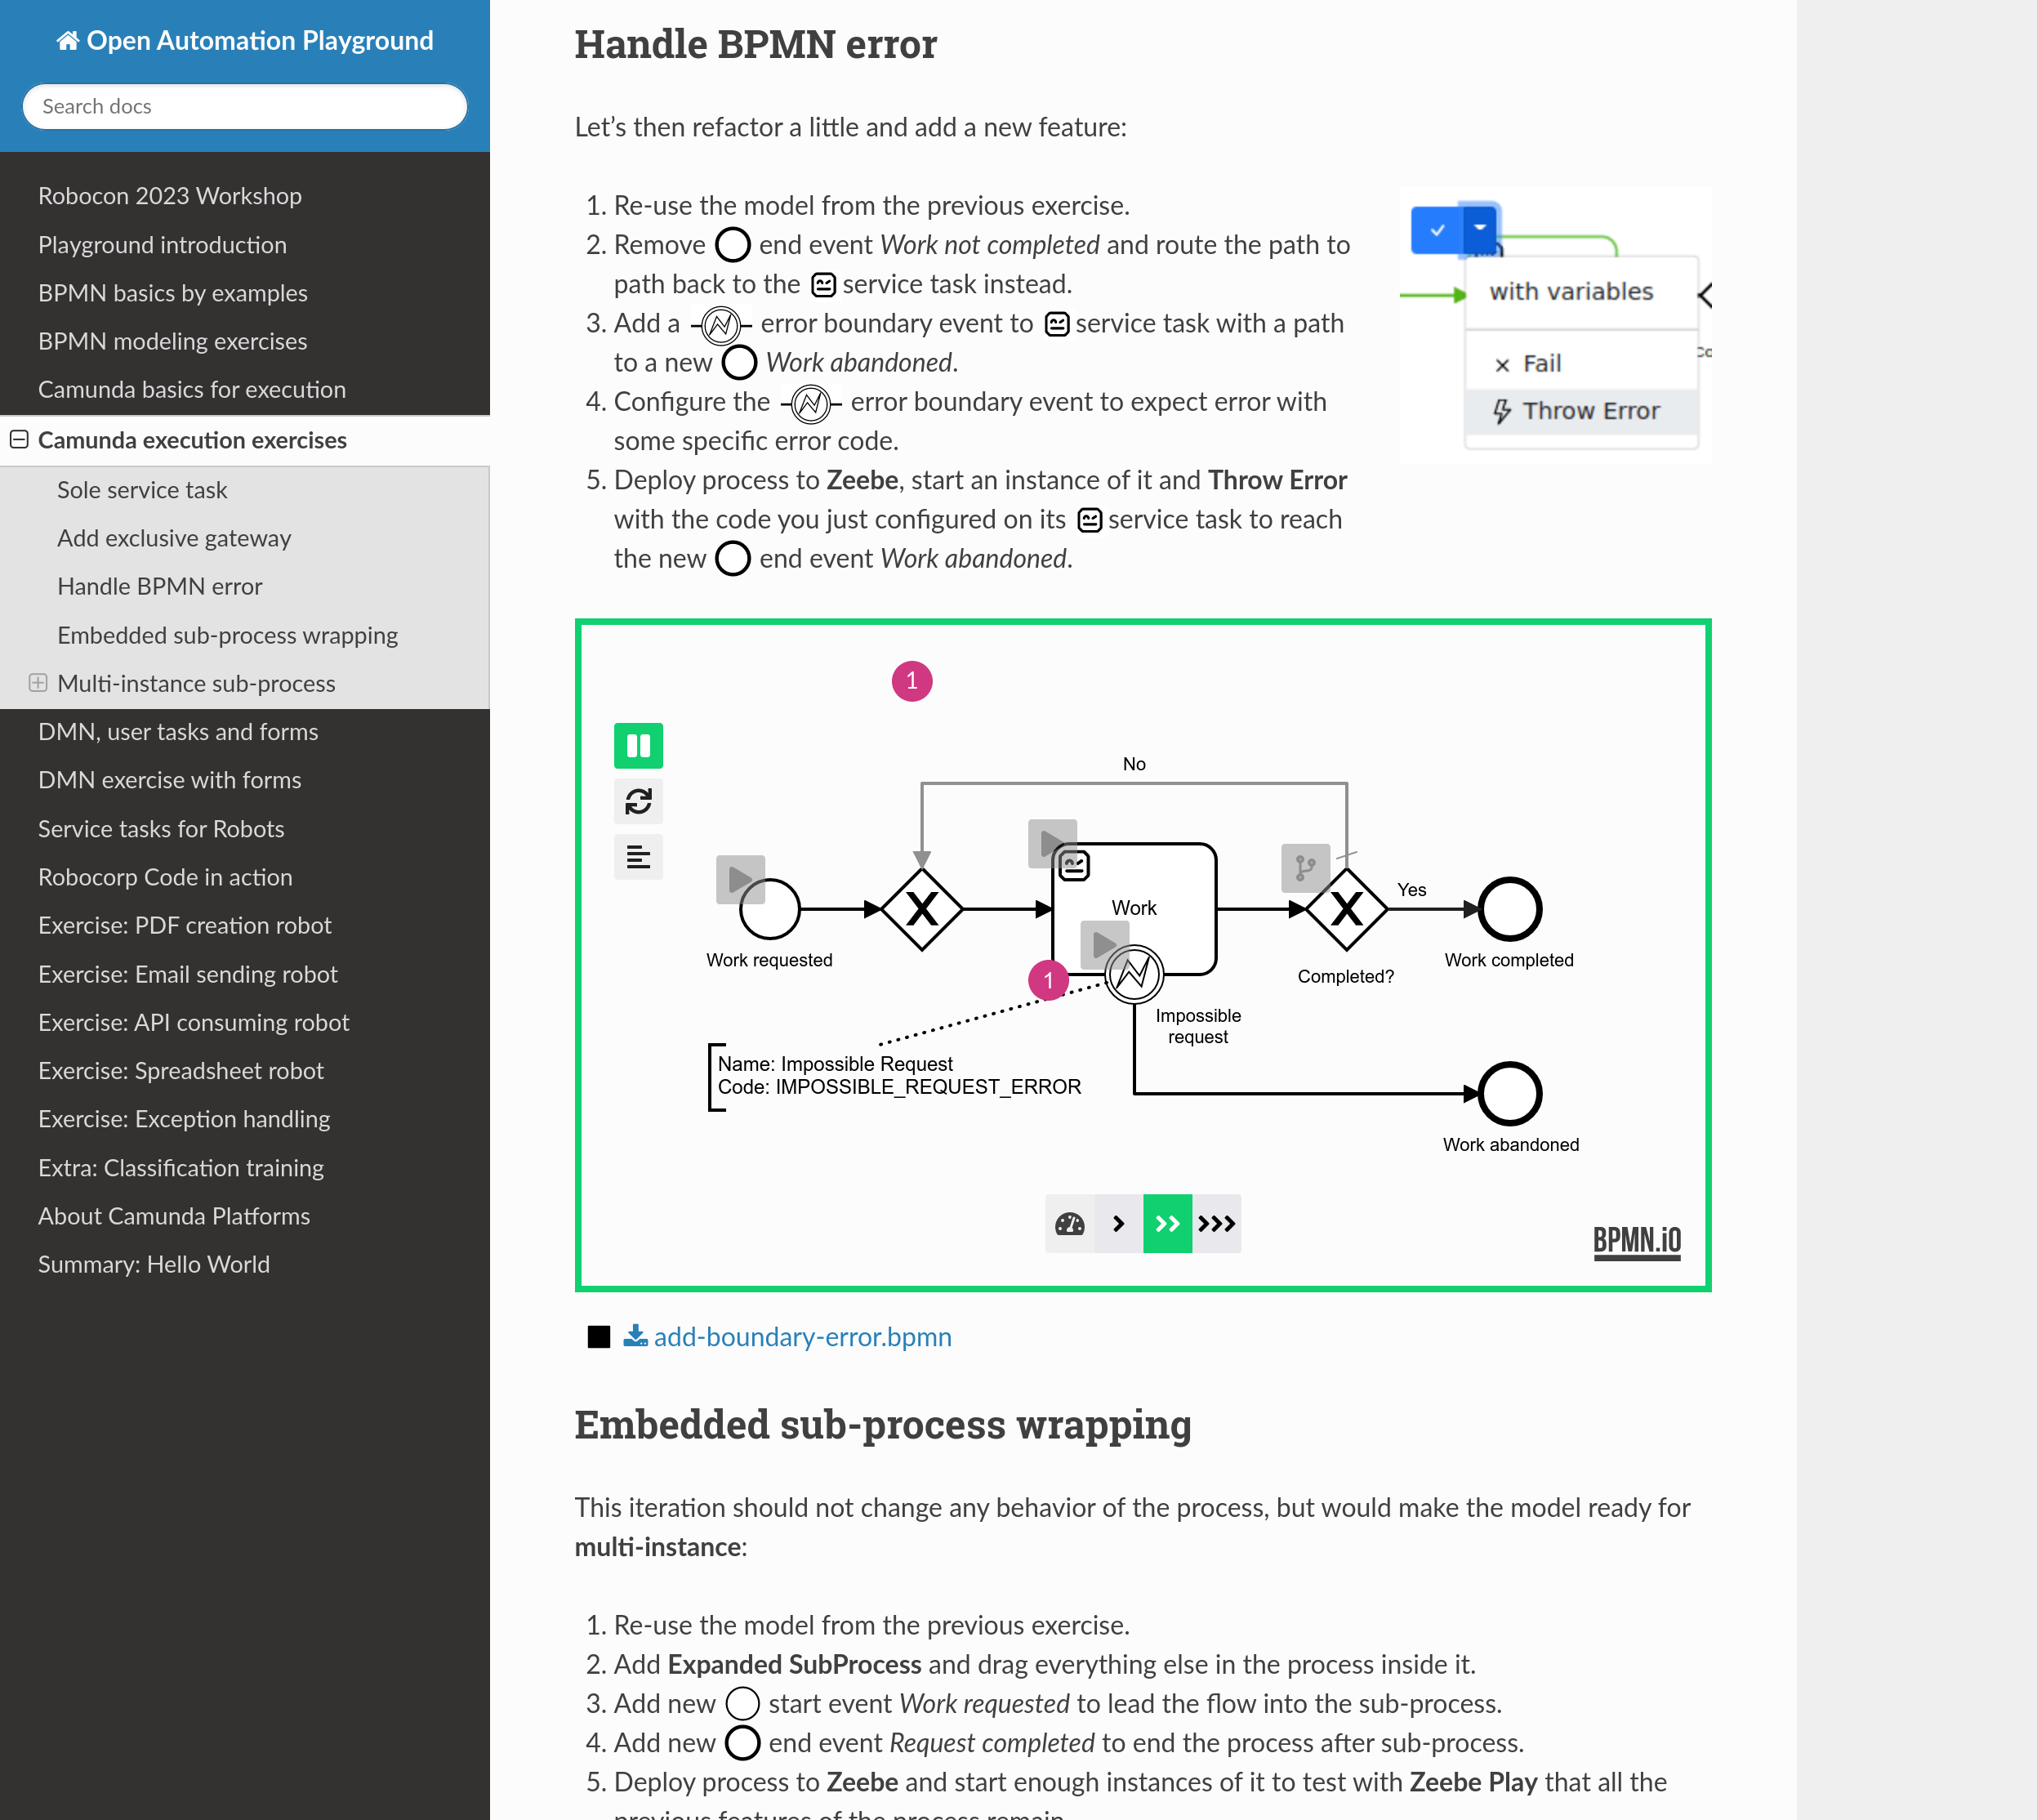
\includegraphics[width=0.8\textwidth]{images/sphinx.png}}
\end{frame}

\section{Camunda 7}

%---------------------------------------------------------------------------------------

\begin{frame}{Camunda 7}
\textbf{Camunda 7 Community Edition}
\par
\vspace{0.5cm}
\par
\begin{minipage}{0.5\textwidth}
\begin{itemize}
    \item License: Apache 2.0
    \item ''Open Core''
    \item Distributions:
\begin{itemize}
    \item \href{https://camunda.com/download/platform-7/}{Camunda Run}
    \item \href{https://camunda.com/download/platform-7/}{Tomcat}
    \item \href{https://hub.docker.com/r/camunda/camunda-bpm-platform}{Docker}
    \item \href{https://start.camunda.com/}{SpringBoot}
    \item \href{https://github.com/camunda-community-hub/micronaut-camunda-platform-7}{Micronaut (unofficial)}
\end{itemize}
\end{itemize}
\end{minipage}
\begin{minipage}{0.45\textwidth}
    \begin{tikzpicture}[remember picture, overlay]
        \node<1> at ([yshift=-1cm, xshift=3cm]current page.center) {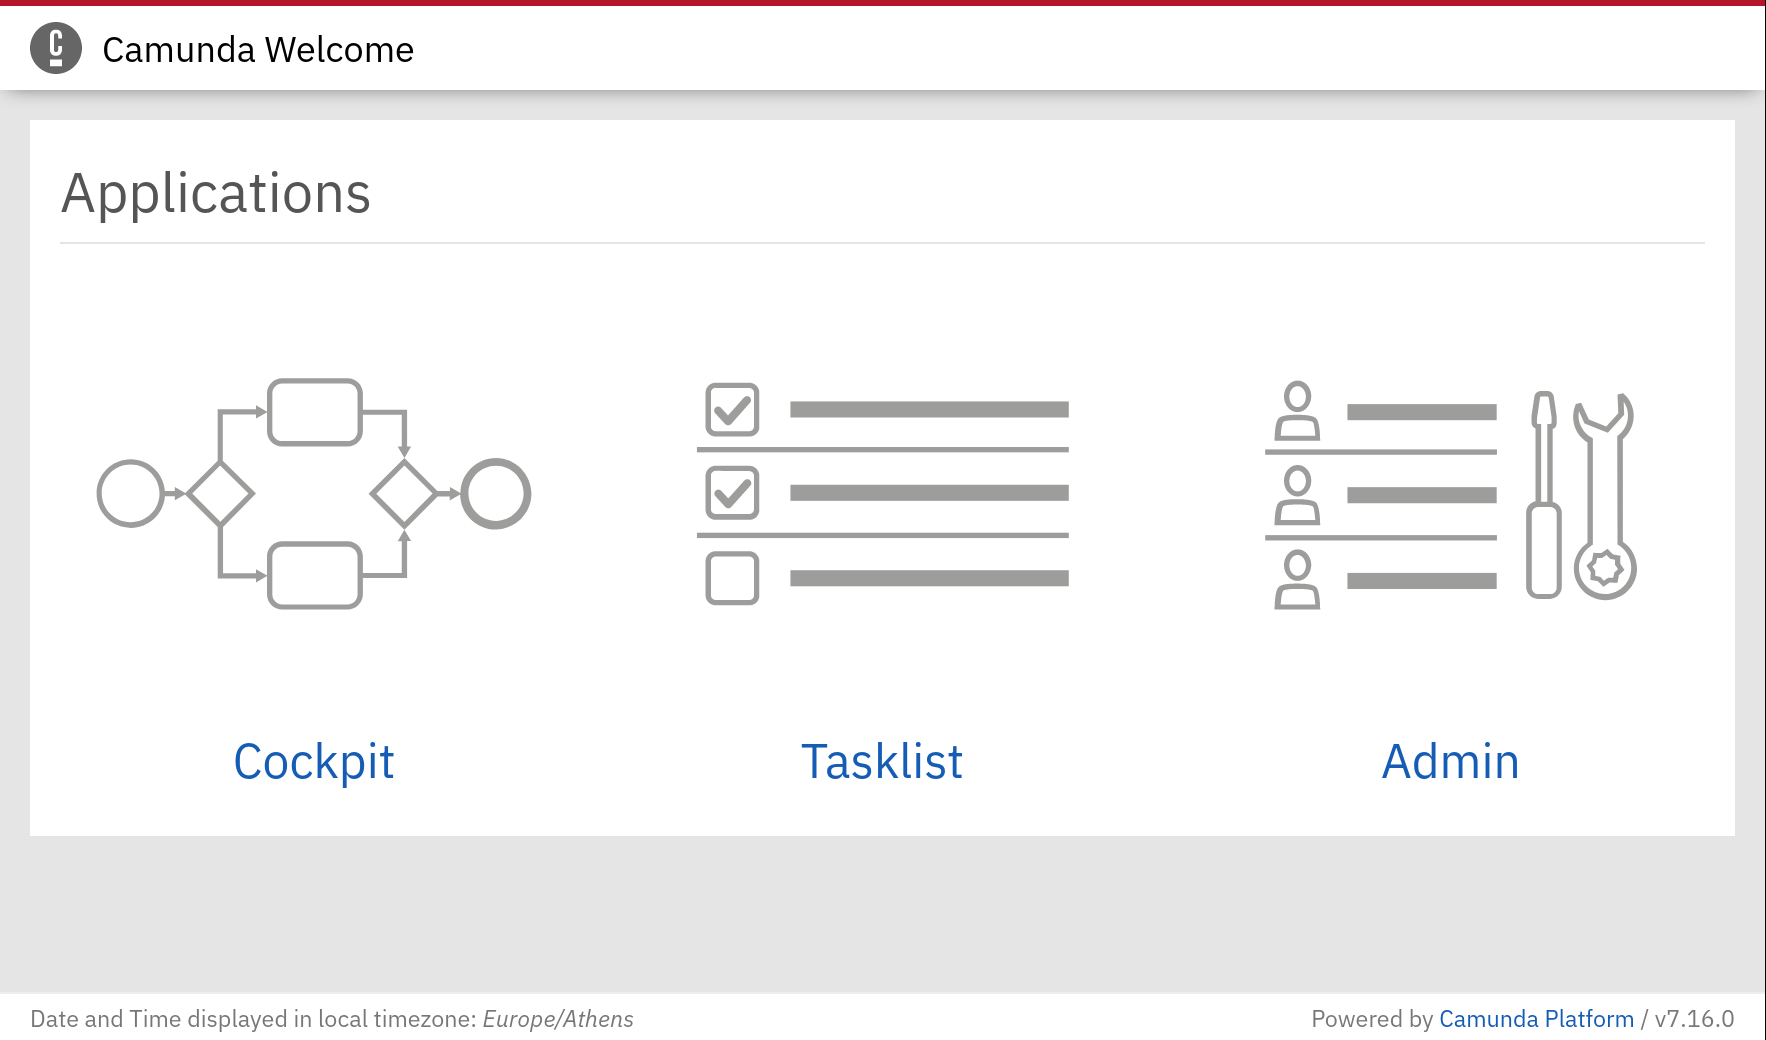
\includegraphics[width=1.2\textwidth]{images/camunda7.png}};
    \end{tikzpicture}
\end{minipage}
\end{frame}

\begin{frame}{Camunda 7 Plugins}
\textbf{Camunda 7 Webapps Plugins}
\par
\vspace{0.5cm}
\par
\begin{minipage}{0.5\textwidth}
\begin{itemize}
    \item \href{https://github.com/datakurre/camunda-cockpit-plugins}{Minimal History}
    \item \href{https://github.com/datakurre/camunda-cockpit-plugin-jupyter}{JupyterLite}
    \item \href{https://github.com/StephenOTT/camunda-formio-plugin}{form.io-forms}
    \item[]
\end{itemize}
\textbf{Other}
\begin{itemize}
    \item \href{https://github.com/StephenOTT/Cammand}{Cammand}
\end{itemize}
\end{minipage}
\begin{minipage}{0.45\textwidth}
    \begin{tikzpicture}[remember picture, overlay]
        \node<1> at ([yshift=-1cm, xshift=2cm]current page.center) {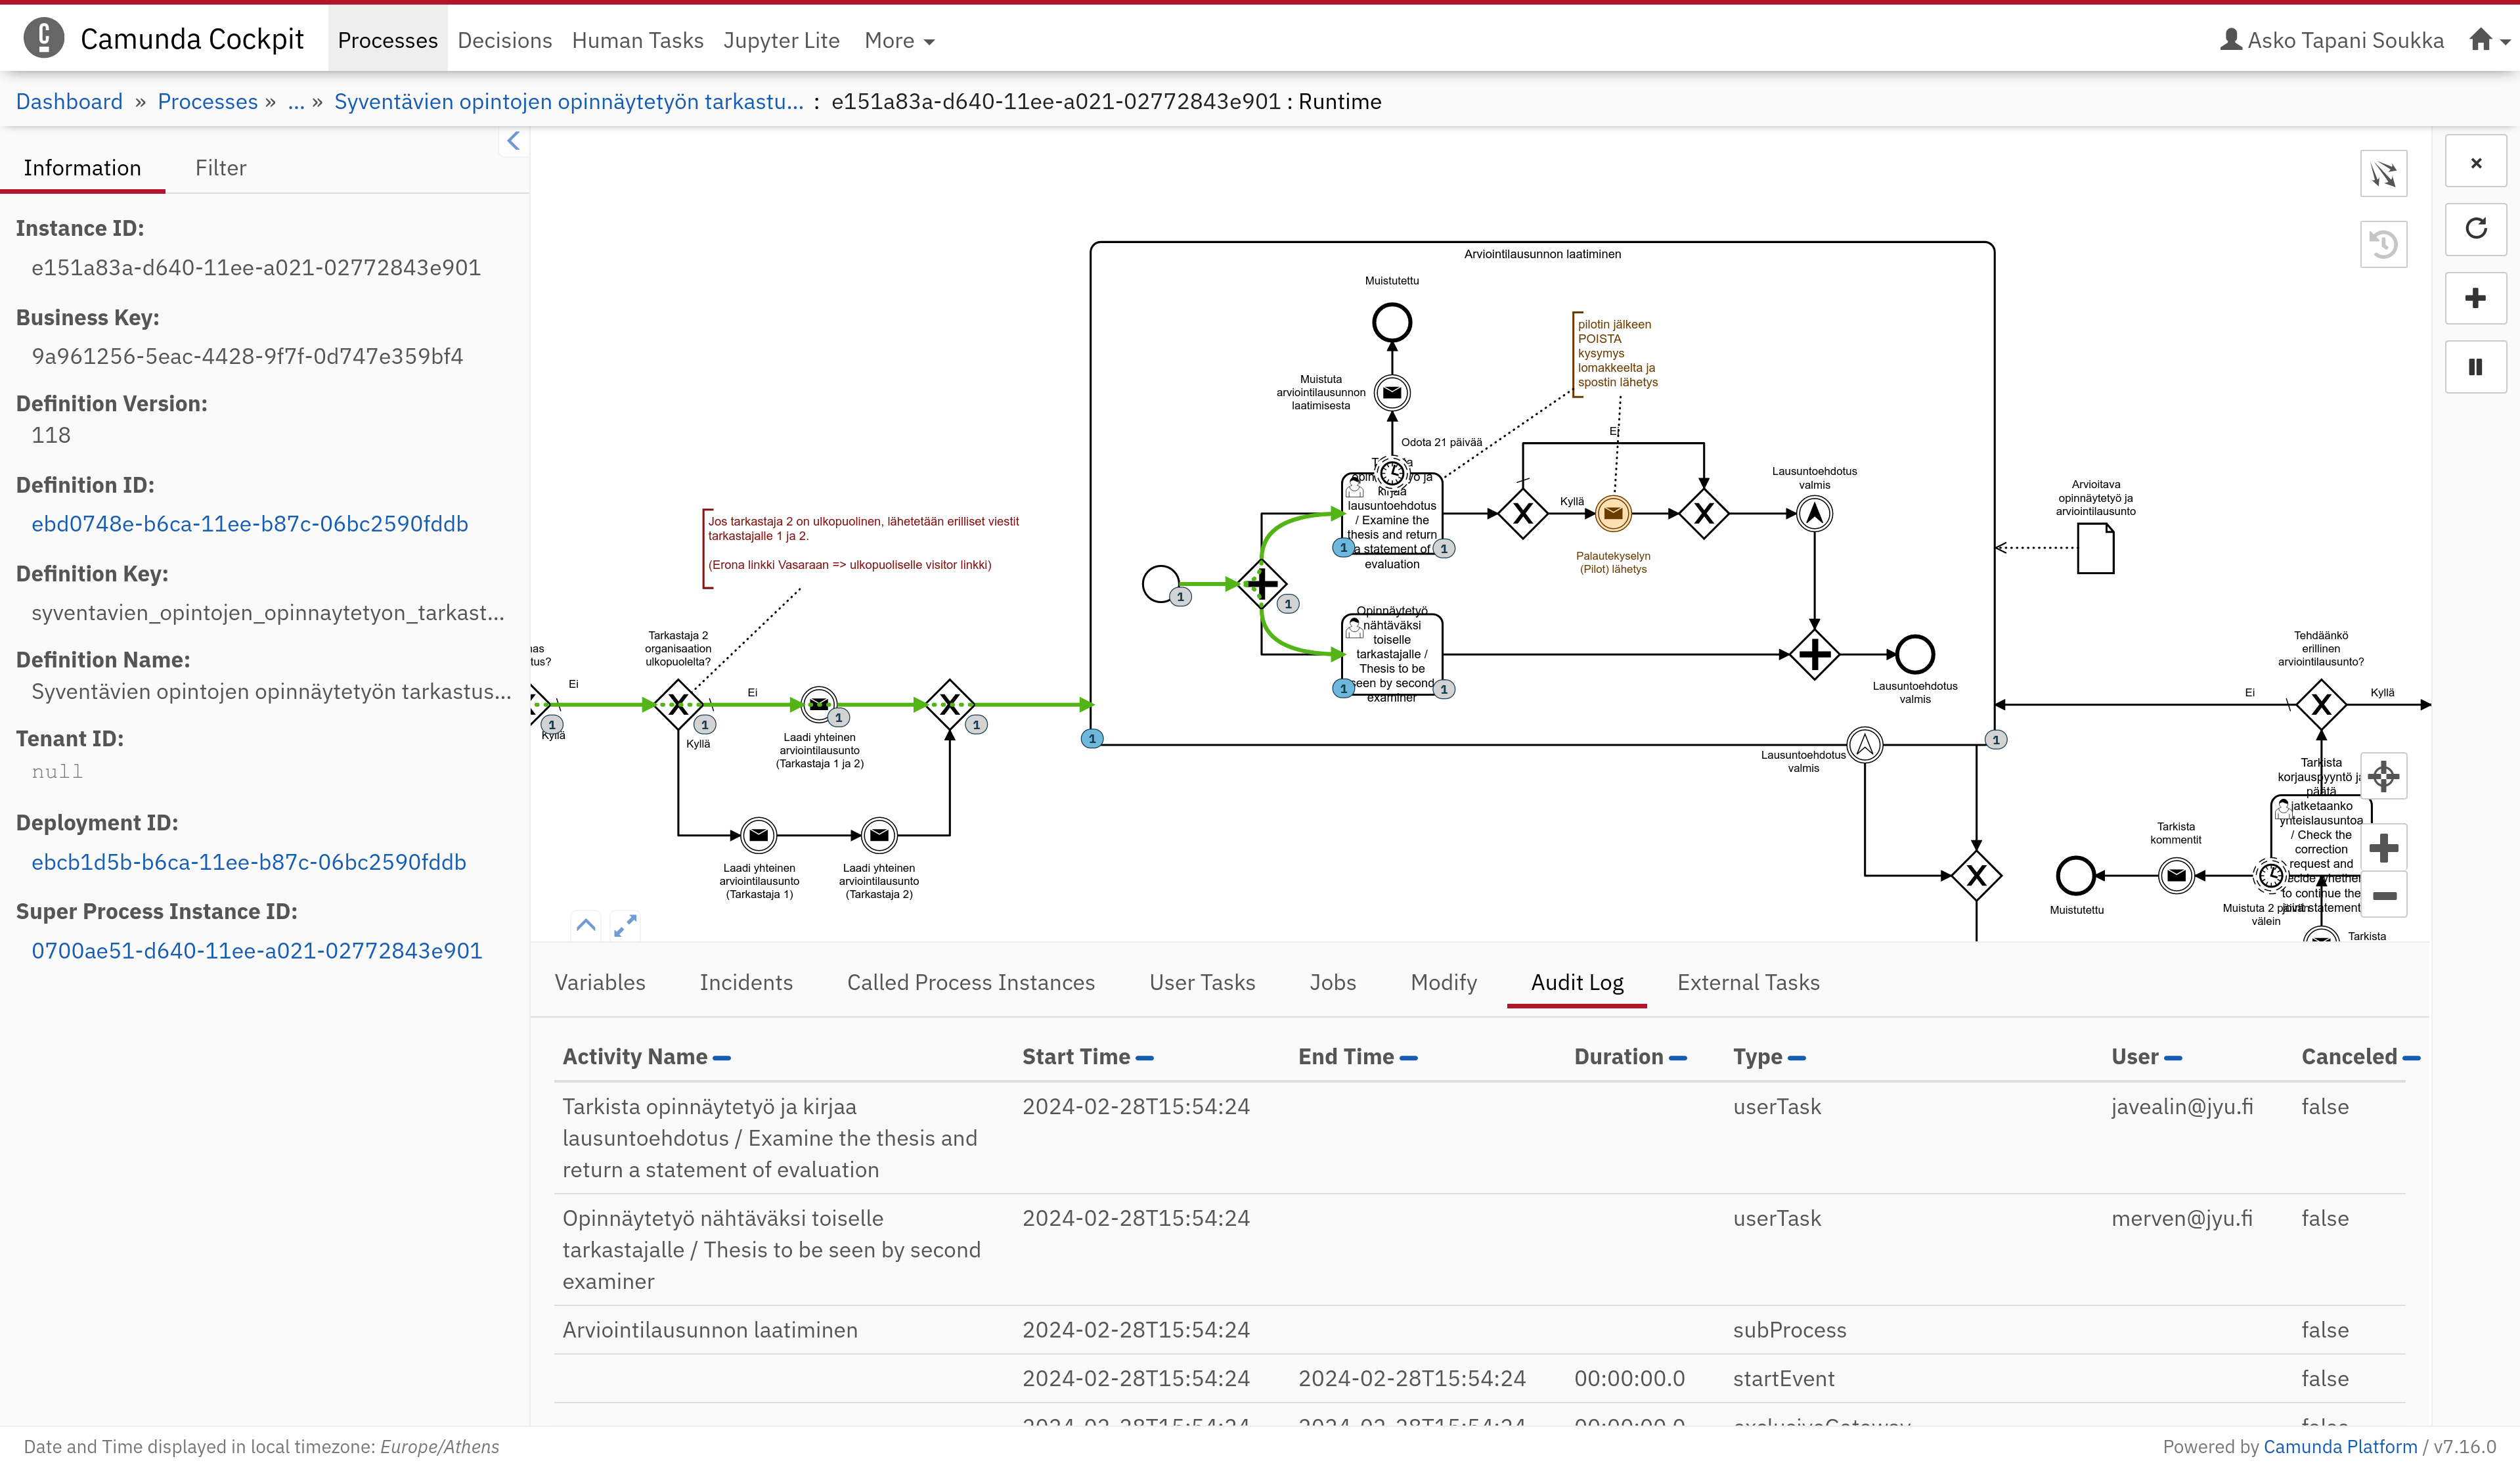
\includegraphics[width=1.2\textwidth]{images/camunda7-plugins.png}};
    \end{tikzpicture}
\end{minipage}
\end{frame}

\begin{frame}{Camunda 7 Plugins}
\textbf{Camunda 7 Backend Plugins}
\begin{itemize}
\item \href{https://github.com/camunda-community-hub/camunda-platform-7-keycloak}{Keycloak Identity Provider}
\item \href{https://github.com/camunda-community-hub/camunda-platform-7-graphql}{GraphQL API}
\end{itemize}
\textbf{Other}
\begin{itemize}
\item \href{https://github.com/camunda-community-hub/awesome-camunda-7-external-clients}{External Task Clients}
\item \href{https://gitlab.com/vasara-bpm/camunda-message-gateway}{Vasara ''Message Gateway''}
\item \href{https://gitlab.com/vasara-bpm/carrot-rcc}{Vasara ''Carrot RCC''}
\end{itemize}
\end{frame}

\begin{frame}{Camunda 7 Platforms}
\textbf{Camunda 7 Based Platforms}
\par
\vspace{0.5cm}
\par
\begin{minipage}{0.5\textwidth}
\begin{itemize}
    \item<1-> \href{https://www.wkspower.com/}{WKS Platform}
    \item<2-> \href{https://digiwf.oss.muenchen.de/}{digiWF}
    \item<3-> \href{https://github.com/AgileKip}{AgileKIP} (on-hold)
    \item<4-> \href{https://digitalstate.io/}{Digital State} (unknown)
    \item<4-> \href{https://gitlab.com/vasara-bpm/vasara}{Vasara} (in-progress)
    \item<4-> \href{https://datakurre.pandala.org/2022/10/collective-bpmproxy/}{Plone-integration} (on-hold)
\end{itemize}
\end{minipage}
\begin{minipage}{0.45\textwidth}
    \begin{tikzpicture}[remember picture, overlay]
        \node<1> at ([yshift=-1cm, xshift=2cm]current page.center) {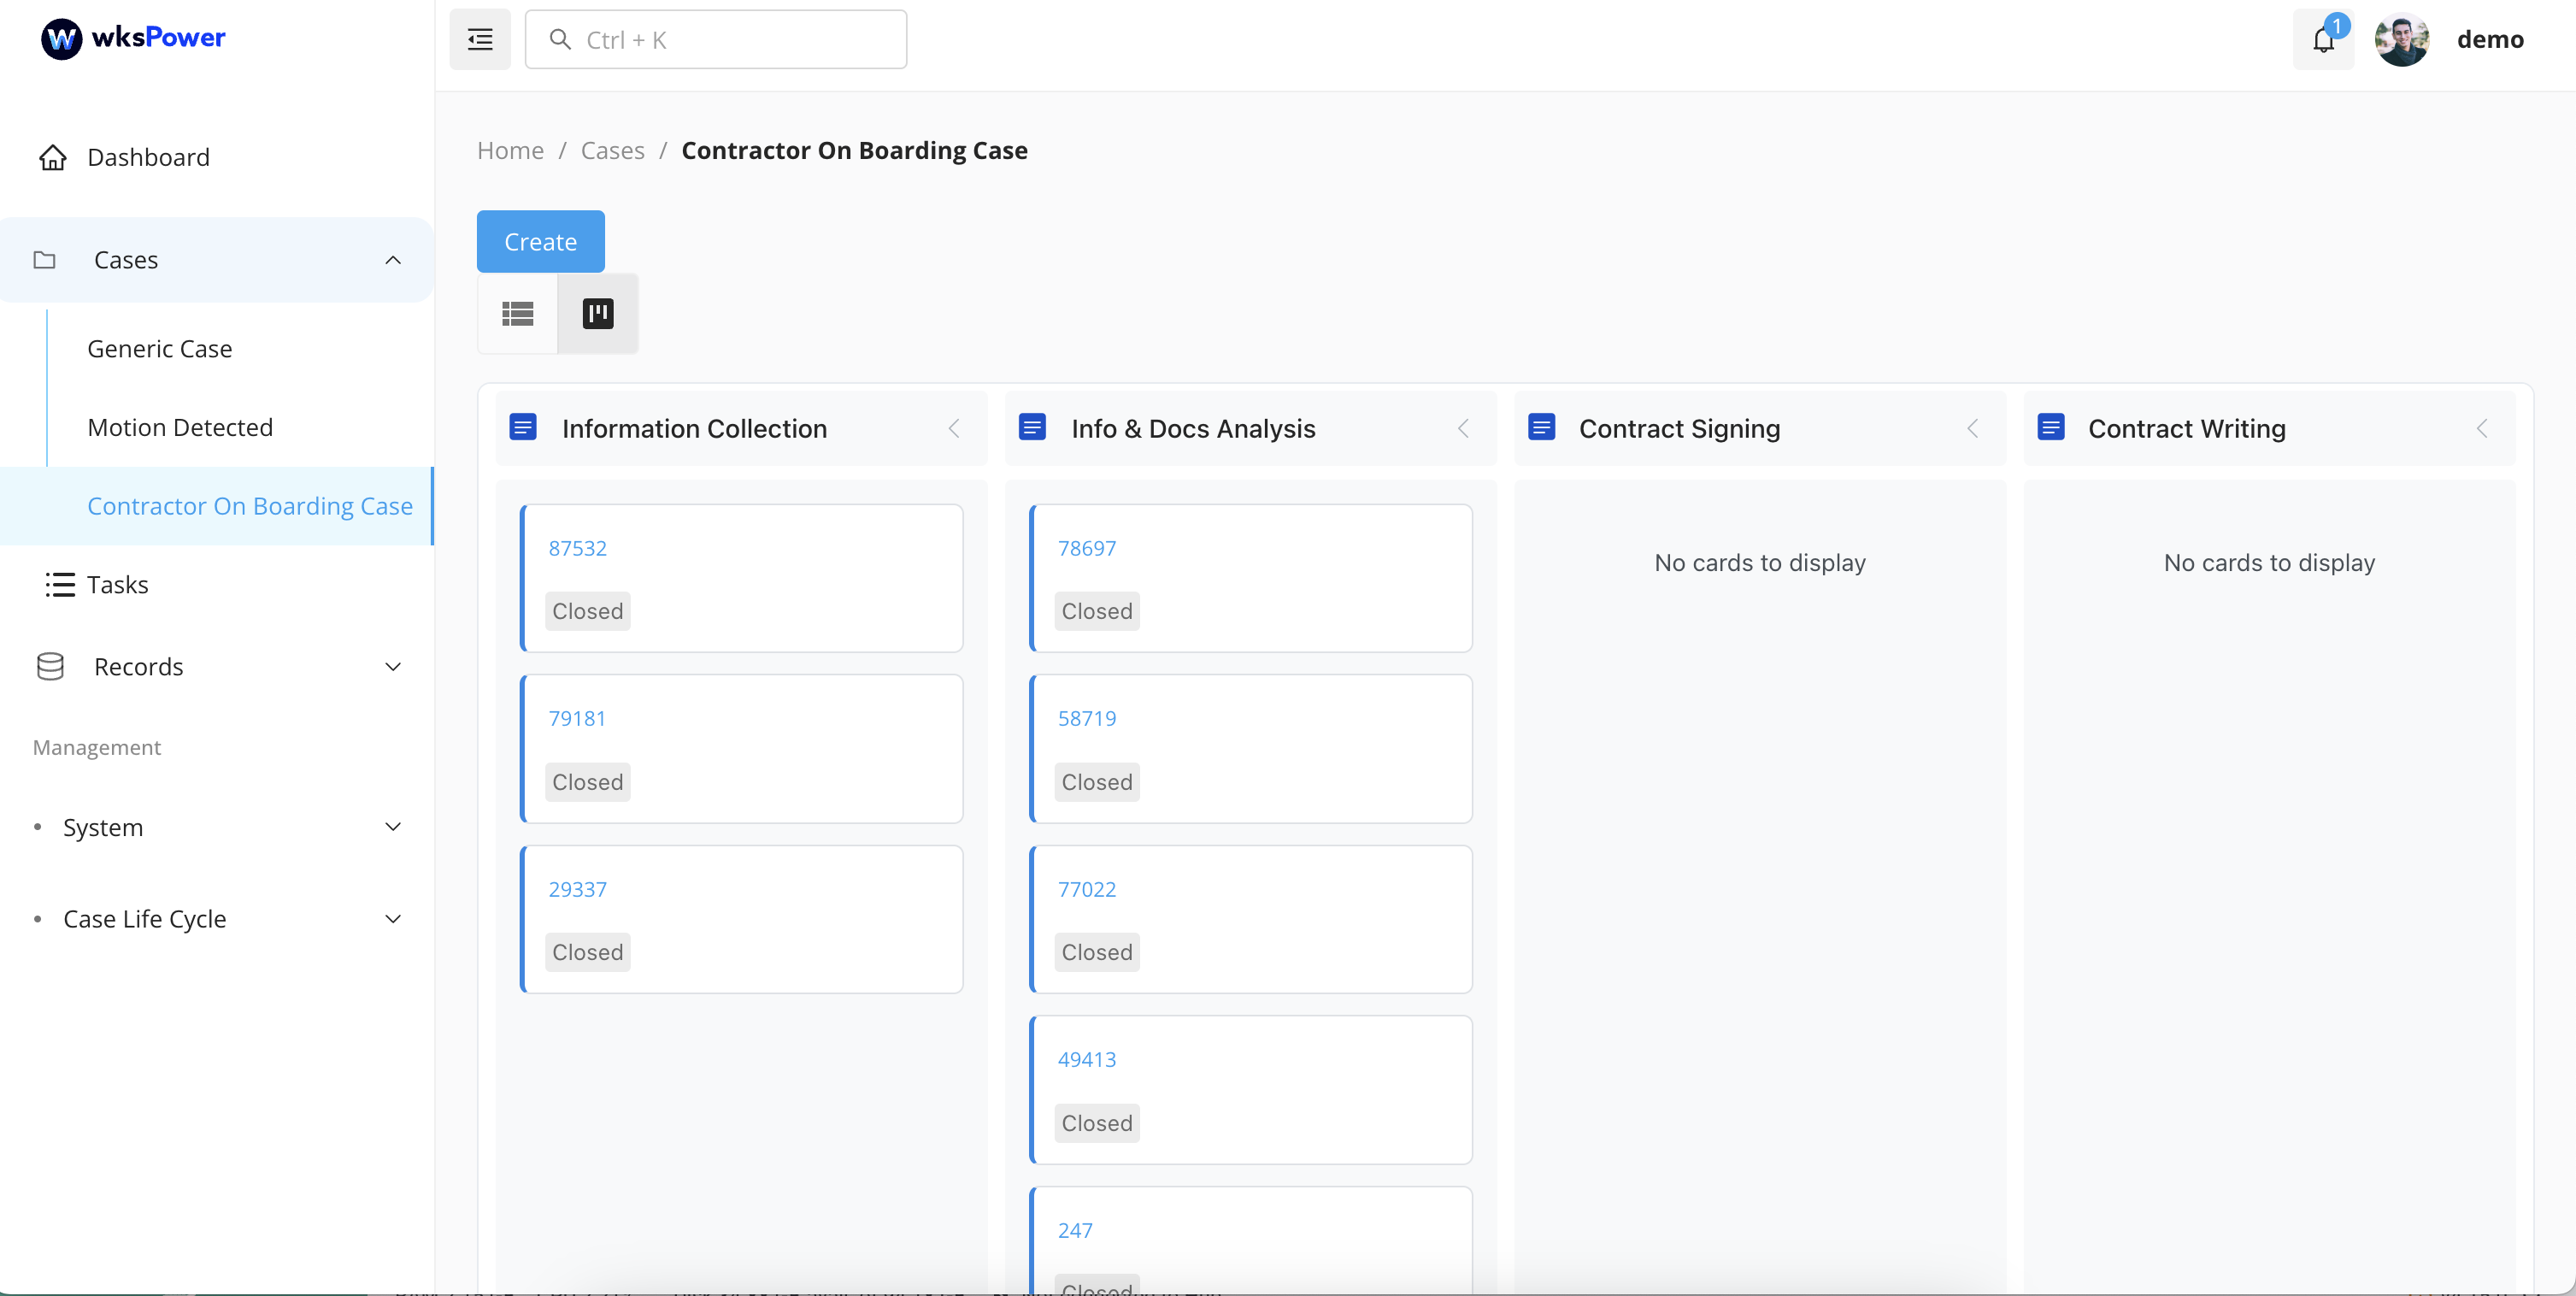
\includegraphics[width=1.4\textwidth]{images/wksplatform.png}};
        \node<2> at ([yshift=-1cm, xshift=2cm]current page.center) {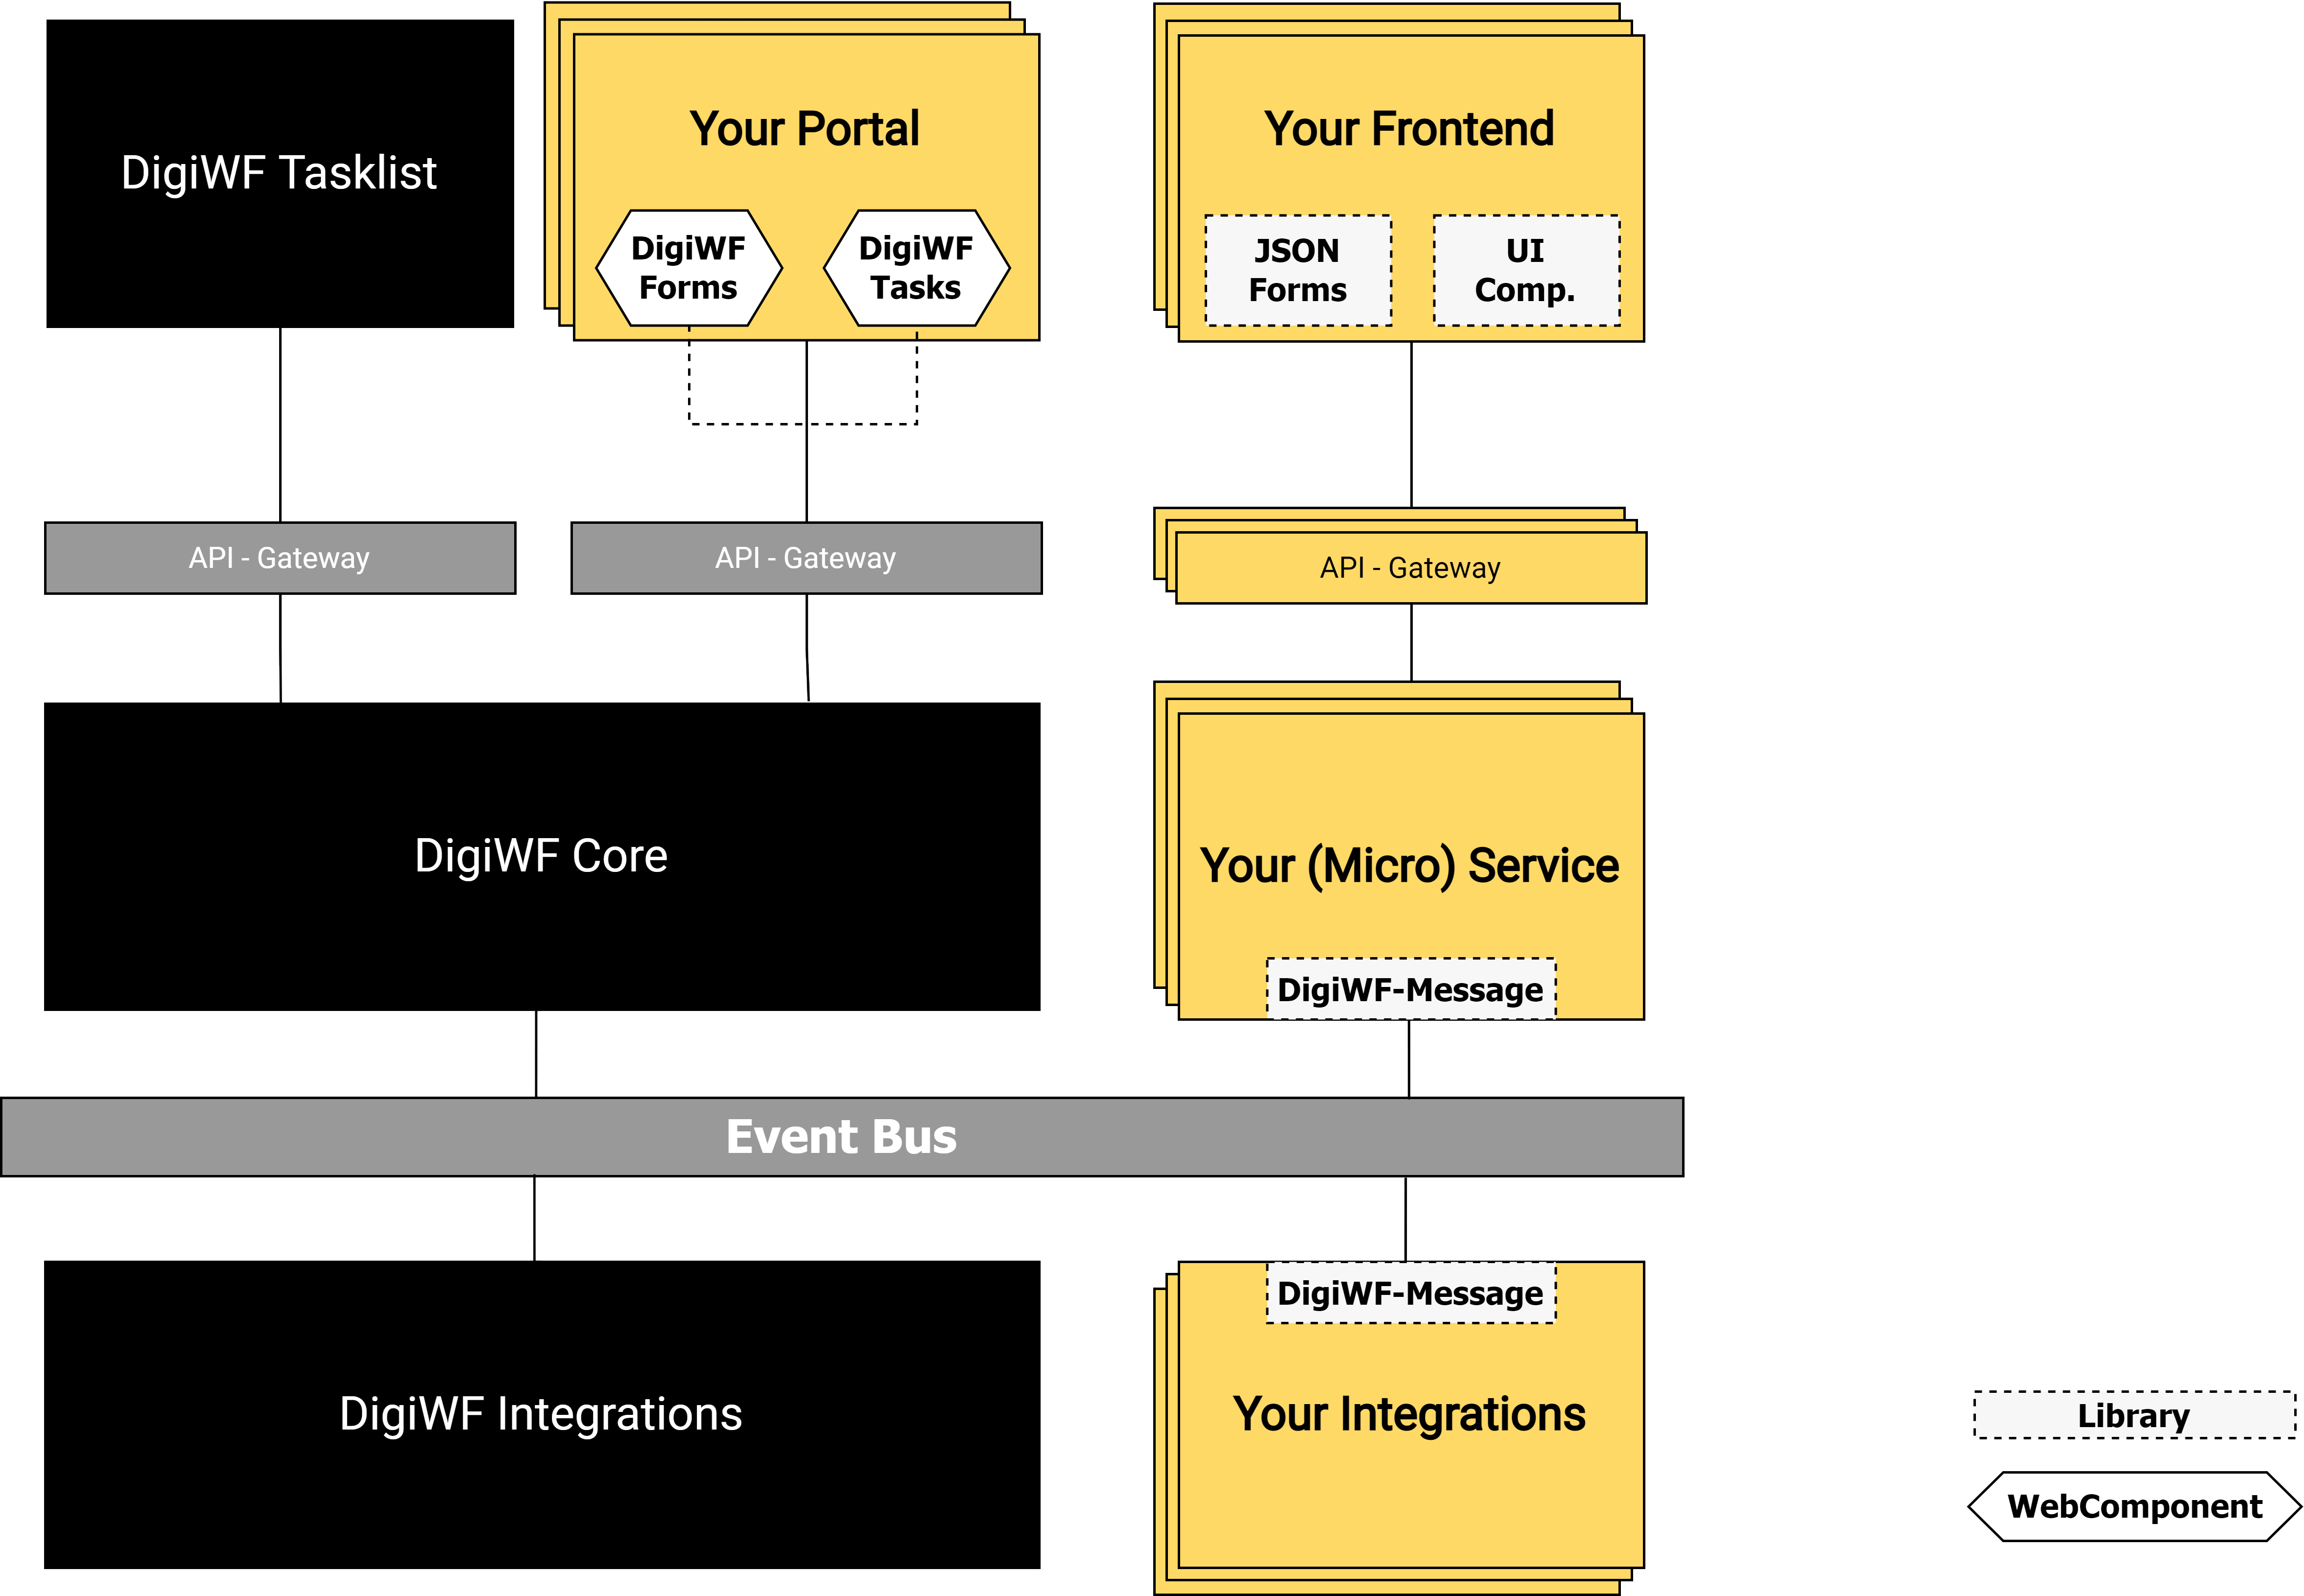
\includegraphics[width=1.2\textwidth]{images/digiwf.png}};
        \node<3> at ([yshift=-1cm, xshift=2cm]current page.center) {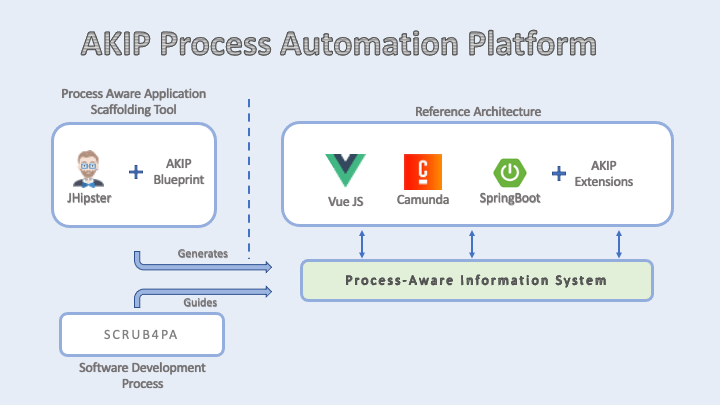
\includegraphics[width=1.2\textwidth]{images/agilekip.png}};
        \node<4> at ([yshift=-1cm, xshift=2cm]current page.center) {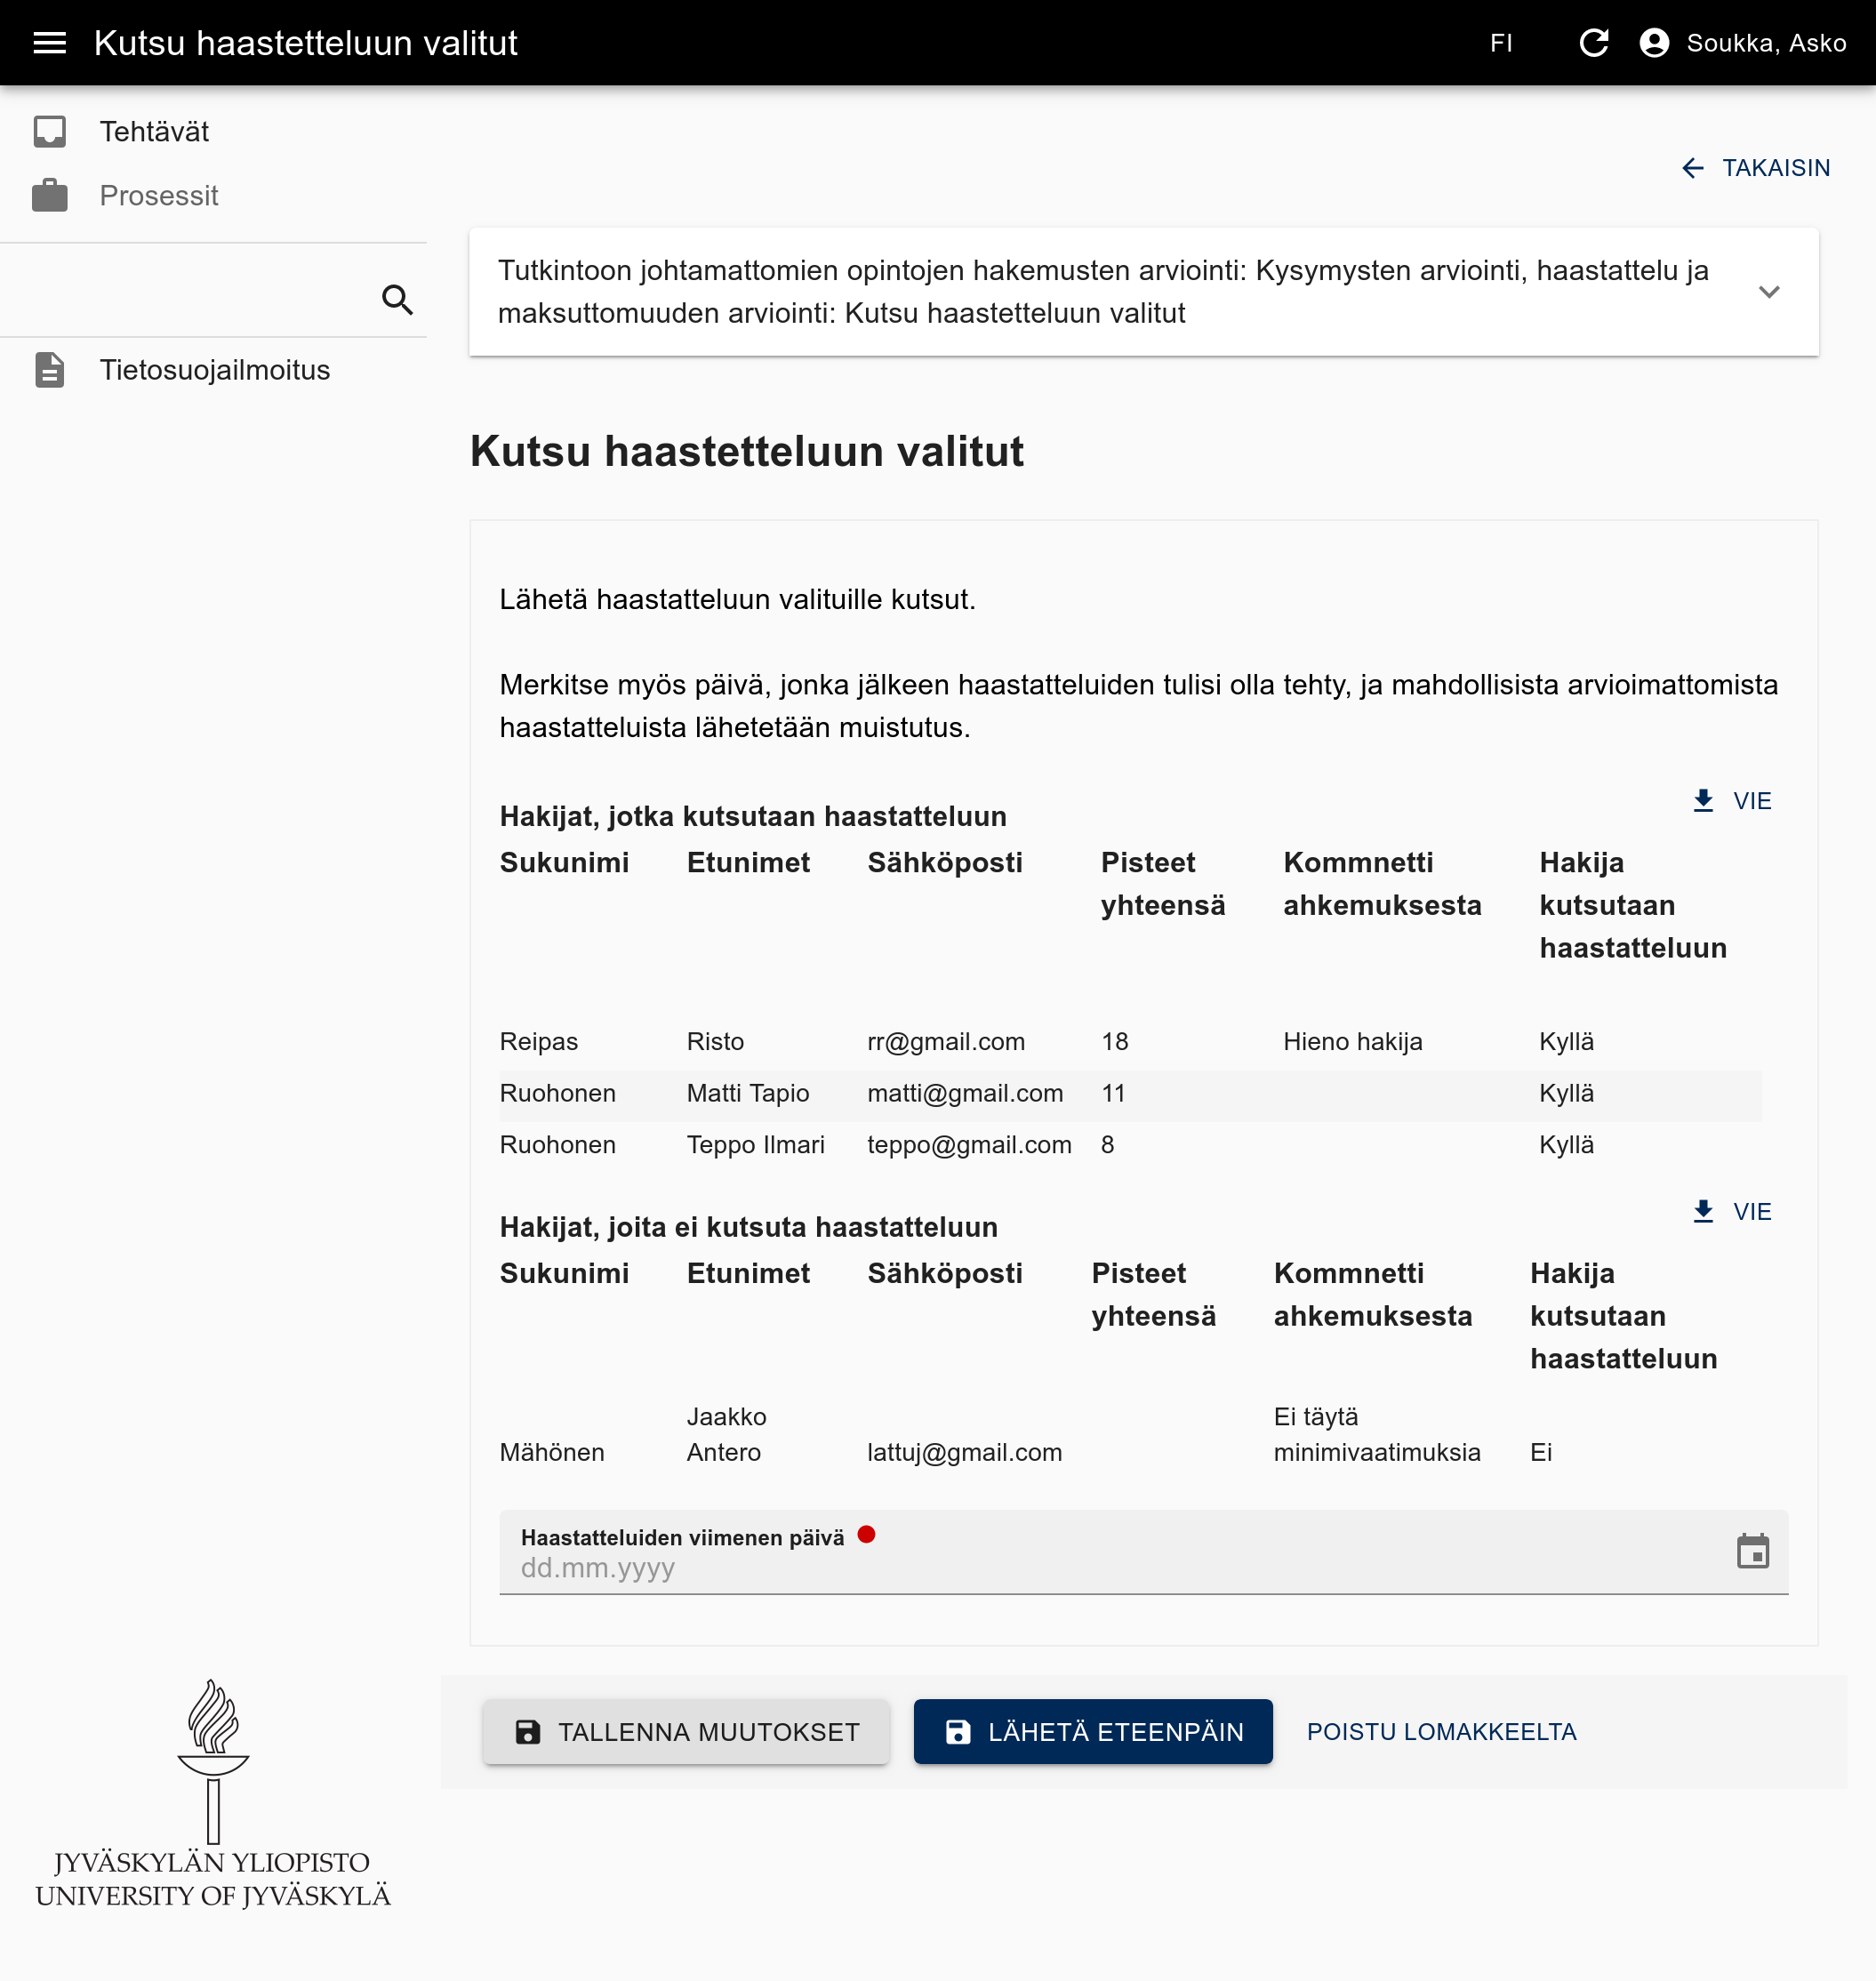
\includegraphics[width=0.8\textwidth]{images/vasara.png}};
    \end{tikzpicture}
\end{minipage}
\end{frame}


\begin{frame}{Camunda 7 EOL}
\begin{itemize}
    \item Camunda 7 CE will EOL (end of life) in October 2025
    \item final release (v7.24), happening on Oct 14, 2025
    \item GitHub repo will be archived, deprecated
    \item artifacts on Maven Central will no longer be maintained
    \item[]
    \item[] \textit{Camunda 7 Enterprise Edition (EE) will EOL in April 2030}
\end{itemize}
\end{frame}

\section{Zeebe (Camunda 8)}

%---------------------------------------------------------------------------------------

\begin{frame}{Camunda 8 Licensing}
\begin{itemize}
\item Zeebe – Zeebe Community License 1.1
\item Connector SDK – Apache 2.0
\item Camunda Webapps – proprietary
\item Camunda Connectors – proprietary
\end{itemize}
\end{frame}

\begin{frame}{Camunda 7 vs. Zeebe}
\par
\vspace{0.5cm}
\par
\begin{minipage}{0.5\textwidth}
\begin{itemize}
    \item[] \textbf{Camunda 7}
    \item[]
    \item Apache 2.0
    \item Full stack
    \item Standalone
    \item Transactional
    \item Integratable
    \item REST API $+$ long-poll
    \item Customizable
\end{itemize}
\end{minipage}
\begin{minipage}{0.45\textwidth}
\begin{itemize}
    \item[] \textbf{Zeebe}
    \item[]
    \item Custom
    \item Only engine
    \item Cluster
    \item Event-driven
    \item External service
    \item gRPC $+$ exporters
    \item Opinionated
\end{itemize}
\end{minipage}
\end{frame}

\begin{frame}{Zeebe OSS ecosystem}
\textbf{\href{https://github.com/camunda-community-hub/awesome-camunda-platform-8}{https://github.com/camunda-community-hub}}
\begin{itemize}
    \item interceptors
    \item exporters
    \item task clients
    \item ''connectors''
    \item APIs
    \item webapps
\end{itemize}
\end{frame}

\begin{frame}{Zeebe OSS picks}
\par
\vspace{0.5cm}
\par
\begin{minipage}{0.5\textwidth}
\begin{itemize}
    \item \href{https://github.com/camunda-community-hub/zeebe-keycloak-interceptor}{zeebe-keycloak-interceptor}
    \item \href{https://gitlab.com/vasara-bpm/zeebe-jwt-interceptor}{zeebe-jwt-interceptor}
    \item \href{https://github.com/camunda-community-hub/zeebe-redis-exporter}{zeebe-redis-exporter}
    \item \href{https://github.com/camunda-community-hub/zeebe-simple-monitor}{zeebe-simple-monitor}
    \item \href{https://github.com/camunda-community-hub/zeeqs}{zeeqs (GraphQL API)}
    \item \href{https://github.com/camunda-community-hub/zeebe-play}{zeebe-play}
    \item \href{https://github.com/datakurre/parrot-rcc}{Parrot RCC}
    \item \href{https://datakurre.pandala.org/2023/04/diy-zeebe-dashboards/}{datasette.io example}
    \item \href{https://github.com/camunda-community-hub/camunda-8-connectors}{Connector SDK Connectors}
\end{itemize}
\end{minipage}
\begin{minipage}{0.45\textwidth}
    \begin{tikzpicture}[remember picture, overlay]
        \node<1> at ([yshift=-0.5cm, xshift=3cm]current page.center) {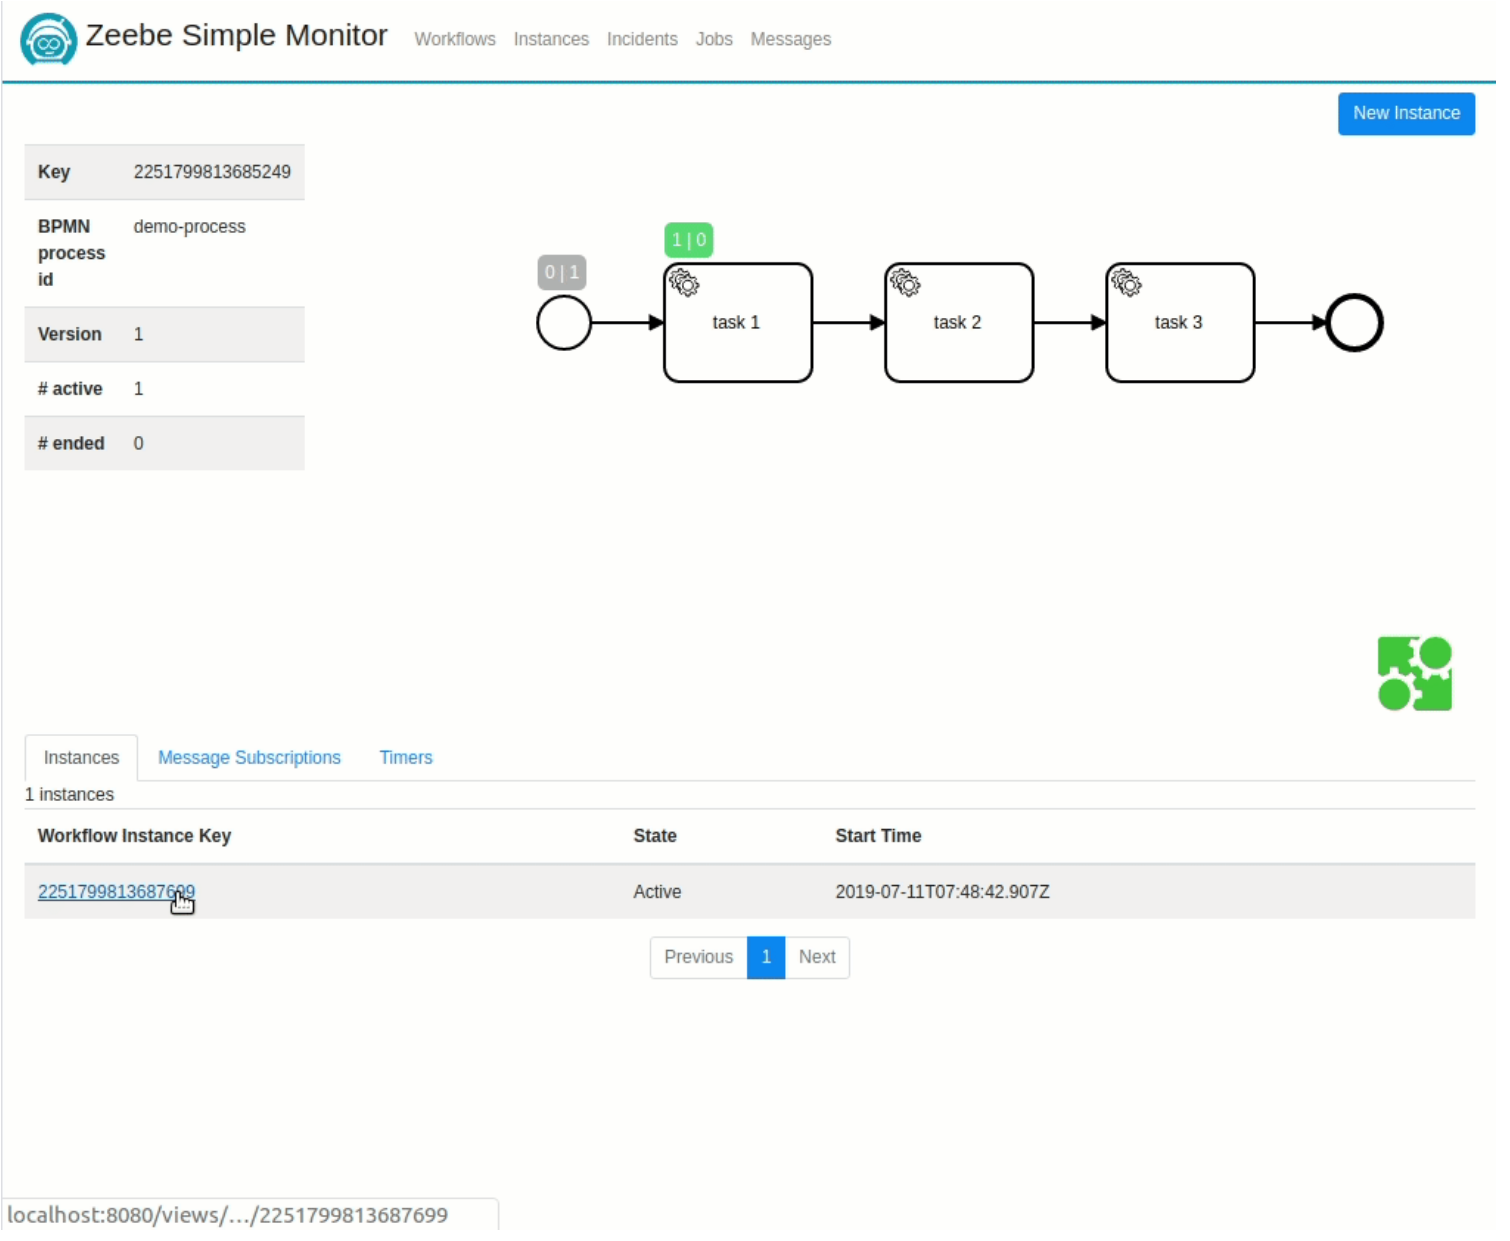
\includegraphics[width=1.2\textwidth]{images/simple-monitor.png}};
    \end{tikzpicture}
\end{minipage}
\end{frame}

\begin{frame}{Zeebe Playground (2022)}
\centering
\textbf{\href{https://datakurre.github.io/automation-playground}{Open Automation Playground}}
\par
{\href{https://datakurre.github.io/automation-playground}{https://datakurre.github.io/automation-playground}}
\end{frame}


\end{document}
